\documentclass[11pt]{article}
\makeatletter\def\input@path{{../}}\makeatother
\usepackage{preamble}
\renewcommand{\chaptername}{Chapter 4: Linear models}
\graphicspath{{figures/}}

% JAGS output for Exercise 9 (ch04/code/ch04_jags.R, run on GitHub Actions).
\newcommand{\JAGSnineTable}{%
\centering
\begin{tabular}{lcccc}\toprule
 & Mean & 95\% interval & $\hat R$ & ESS (of 90{,}000)\\\midrule
$\alpha$ & $-10.9$ & $(-166,\ 140)$ & 1.006 & 920\\
$\beta$ & 0.082 & $(-0.27,\ 0.44)$ & 1.011 & 580\\
$\rho$ & 0.987 & $(0.913,\ 0.9998)$ & 1.006 & 599\\
$\sigma$ & 0.181 & $(0.152,\ 0.216)$ & 1.000 & 77{,}870\\\bottomrule
\end{tabular}\par\smallskip\raggedright
Same posterior as our sampler. Note the much smaller ESS for $\alpha,\beta,\rho$ in JAGS: our Gibbs sampler updates $(\alpha,\beta)$ \emph{jointly} given $\rho$, which removes their strong posterior correlation, whereas JAGS updates them one at a time.}
\newcommand{\JAGSexnine}{%
\begin{sanity}\small\textbf{JAGS output} (run on GitHub Actions; 3 chains $\times$ 30{,}000 draws).\par\smallskip
\JAGSnineTable
\end{sanity}}

\begin{document}

\solutionstitlepage{4}{Linear models}{All numbers and figures are reproduced by \texttt{ch04/code/ch04.R} (hand-written Gibbs and Metropolis samplers, base R). The JAGS version of Exercise 9 is in \texttt{ch04/code/ch04\_jags.R} and runs on GitHub. Data sources are listed in \texttt{data/README.md}.}

\tableofcontents
\clearpage

\section*{Answers at a glance}
\addcontentsline{toc}{section}{Answers at a glance}
\begin{center}
\small
\renewcommand{\arraystretch}{1.25}
\begin{tabular}{>{\bfseries\color{navy}}r p{0.82\linewidth}}\toprule
1  & Treatment lowers weight by $\approx2.4$ lb, $\Prob(\delta<0)\approx0.97$; conclusion weakens under sceptical priors.\\
2  & Bayes $\approx$ OLS under vague priors; LASSO shrinks \texttt{indus}, \texttt{age}, \texttt{rad}, \texttt{tax}; predictions for rows 501--506 run high.\\
3  & Education is the strongest predictor; residuals heavy-tailed (Utah/Idaho); state effects cut $\sigma$ from 3.9 to 2.7.\\
4  & Each extra law: $-1.4\%$ deaths (Poisson); NB widens intervals; 0 vs 25 laws: $\approx34{,}500$ vs $24{,}400$ --- not trustworthy.\\
5  & Female OR $\approx12.7$; 2nd/3rd class OR $0.27/0.075$; each 10 years of age OR $0.69$.\\
6  & Gamma GLM: mass grows $\approx22\%$ per year (95\% CI 7--38\%).\\
7  & $\alpha_1\mid\cdot$ normal; $\sigma^2\mid\cdot$, $\tau^2\mid\cdot$ inverse-gamma (Gibbs).\\
8  & Bed nets cut malaria odds; village effects ($\tau\approx0.8$) widen the location-level coefficients.\\
9  & $\rho\approx0.99$ (near random walk); 2020 share of babies named Sophia $\approx1.0\%$ (0.5--1.9\%).\\
10 & $g(2020)-g(1980)\approx0.80^\circ$C (0.69--0.91).\\
11 & Jeffreys: big $n$, few $p$, objective; LASSO: many candidate $p$; informative: small new study + strong prior knowledge.\\
12 & Sparse (spike-and-slab / horseshoe) regression; report posterior inclusion probabilities with FDR control.\\
13 & A 3-component mixture captures the main clusters far better than one $t$ or Laplace.\\
14 & Logistic (occupancy) model with observer and path random effects.\\\bottomrule
\end{tabular}
\end{center}
\clearpage

% ================================================================= primer
\section*{A five-minute primer on the tools of this chapter}
\addcontentsline{toc}{section}{Primer: the tools of this chapter}

\begin{recall}
\textbf{1. Bayesian linear regression.} $\mathbf Y=\mathbf X\bm\beta+\bm\varepsilon$, $\varepsilon_i\iid\dist N(0,\sigma^2)$, with priors $\beta_j\sim\dist N(0,c^2)$ and $\sigma^2\sim\dist{InvGamma}(a,b)$. Gibbs sampler:
\[
\bm\beta\mid\sigma^2,\mathbf Y\sim\dist N\Big(\mathbf V\frac{\mathbf X^\top\mathbf Y}{\sigma^2},\ \mathbf V\Big),\qquad \mathbf V=\Big(\frac{\mathbf X^\top\mathbf X}{\sigma^2}+\frac{\mathbf I}{c^2}\Big)^{-1},
\]
\[
\sigma^2\mid\bm\beta,\mathbf Y\sim\dist{InvGamma}\Big(a+\frac n2,\ b+\frac{\|\mathbf Y-\mathbf X\bm\beta\|^2}{2}\Big).
\]
With $c$ large, the posterior mean $\approx$ the least-squares estimate.

\medskip
\textbf{2. Standardising covariates.} Using $(X_j-\bar X_j)/\mathrm{sd}(X_j)$ puts every coefficient on the same scale (``change in $Y$ per standard deviation of $X_j$''), makes vague priors comparable across covariates and improves MCMC mixing.

\medskip
\textbf{3. Generalised linear models.} Logistic: $\mathrm{logit}\,\Prob(Y_i=1)=\mathbf X_i\bm\beta$ ($e^{\beta_j}$ = odds ratio). Poisson: $\log\E(Y_i)=\log N_i+\mathbf X_i\bm\beta$ ($e^{\beta_j}$ = rate ratio; $\log N_i$ is an \emph{offset}). No conjugate prior exists, so we use \textbf{block random-walk Metropolis} with proposal covariance $\frac{2.4^2}{p}\times$(the classical GLM covariance) --- a standard, well-tuned default.

\medskip
\textbf{4. Random effects.} $Y_{ij}=\mathbf X_{ij}\bm\beta+\alpha_i+\varepsilon_{ij}$ with $\alpha_i\iid\dist N(\mu,\tau^2)$: observations in the same group share $\alpha_i$, so they are correlated. The model ``borrows strength'': groups with little data are shrunk toward $\mu$. We let the random effects have mean $\mu$ (instead of a separate intercept) --- \emph{hierarchical centring} --- which makes the sampler mix much better.

\medskip
\textbf{5. Posterior predictive distribution (PPD).} For each posterior draw $(\bm\beta^{(s)},\sigma^{(s)})$ simulate a new $Y^{*(s)}\sim f(y\mid\bm\beta^{(s)},\sigma^{(s)})$. The collection $\{Y^{*(s)}\}$ is a sample from the PPD; it includes both parameter uncertainty and observation noise.
\end{recall}

\clearpage

% ================================================================= Exercise 1
\exercise{4.1 --- Does the weight-loss drug work?}

\begin{problem}{1}
A clinical trial gave six subjects a placebo and six subjects a new weight loss medication. The response variable is the change in weight (pounds) from baseline (so $-2.0$ means the subject lost 2 pounds). The data for the 12 subjects are:
\begin{center}
\begin{tabular}{cc}\toprule Placebo & Treatment\\\midrule 2.0 & $-3.5$\\ $-3.1$ & $-1.6$\\ $-1.0$ & $-4.6$\\ 0.2 & $-0.9$\\ 0.3 & $-5.1$\\ 0.4 & 0.1\\\bottomrule\end{tabular}
\end{center}
Conduct a Bayesian analysis to compare the means of these two groups. Would you say the treatment is effective? Is your conclusion sensitive to the prior?
\end{problem}

\begin{restate}
Compare the average weight change in the two groups, decide whether the drug really lowers weight, and check whether that conclusion depends on the prior.
\end{restate}

\begin{recall}
\textbf{Two-sample normal model} (Section 4.1.2): $Y_{gi}\sim\dist N(\mu_g,\sigma^2)$, $g\in\{P,T\}$. With the Jeffreys prior $\pi(\mu_P,\mu_T,\sigma^2)\propto1/\sigma^2$,
\[
\delta=\mu_T-\mu_P\mid\mathbf Y\ \sim\ t_{n_P+n_T-2}\Big(\bar Y_T-\bar Y_P,\ s_p^2\big(\tfrac1{n_P}+\tfrac1{n_T}\big)\Big),\qquad s_p^2=\frac{(n_P-1)s_P^2+(n_T-1)s_T^2}{n_P+n_T-2}.
\]
If the variances may differ, each mean has its own posterior $\mu_g\mid\mathbf Y\sim t_{n_g-1}(\bar Y_g,\ s_g^2/n_g)$, and we get $\delta$ by Monte Carlo.
\end{recall}

\begin{keyidea}
``Is the treatment effective?'' becomes ``what is $\Prob(\delta<0\mid\mathbf Y)$?'' (negative $\delta$ = more weight lost). Sensitivity: repeat with increasingly \emph{sceptical} priors $\delta\sim\dist N(0,\tau^2)$ that favour ``no effect''.
\end{keyidea}

\solution
\step{Step 1 --- summary statistics.}
$\bar Y_P=\frac{2.0-3.1-1.0+0.2+0.3+0.4}{6}=-0.200$ and $\bar Y_T=\frac{-3.5-1.6-4.6-0.9-5.1+0.1}{6}=-2.600$, so $\bar Y_T-\bar Y_P=-2.400$. Pooled SD $s_p=1.921$, standard error $s_p\sqrt{\frac16+\frac16}=1.109$.

\step{Step 2 --- equal-variance posterior.}
$\delta\mid\mathbf Y\sim t_{10}(-2.400,\ 1.109^2)$. 95\% interval $-2.400\pm t_{10,0.975}\times1.109=-2.400\pm2.228\times1.109=(-4.87,\ 0.07)$, and
\[
\Prob(\delta<0\mid\mathbf Y)=\Prob\Big(t_{10}<\frac{0-(-2.400)}{1.109}\Big)=\Prob(t_{10}<2.164)=0.972.
\]
\step{Step 3 --- unequal variances (Monte Carlo).}
Draw $\mu_P$ and $\mu_T$ from their own $t$ posteriors ($10^6$ times) and subtract: mean $-2.40$, 95\% interval $(-5.25,\ 0.45)$, $\Prob(\delta<0)=0.957$.
\begin{center}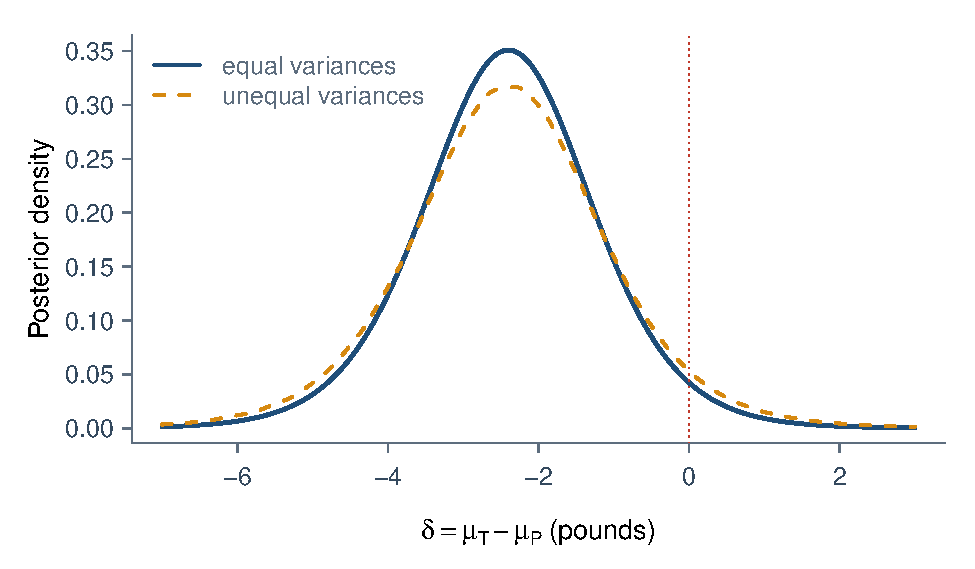
\includegraphics[width=0.7\linewidth]{ex01_delta.pdf}\end{center}

\step{Step 4 --- sensitivity to the prior on $\delta$.}
Gibbs sampler (Exercise 3.5 style) with $\delta\sim\dist N(0,\tau^2)$:
\begin{center}
\begin{tabular}{cccc}\toprule
Prior SD $\tau$ & Posterior mean of $\delta$ & 95\% interval & $\Prob(\delta<0\mid\mathbf Y)$\\\midrule
100 (vague) & $-2.39$ & $(-4.88,\ 0.13)$ & 0.970\\
10 & $-2.38$ & $(-4.84,\ 0.04)$ & 0.973\\
2 & $-1.77$ & $(-3.74,\ 0.39)$ & 0.950\\
1 & $-0.99$ & $(-2.53,\ 0.68)$ & 0.886\\
0.5 & $-0.34$ & $(-1.27,\ 0.62)$ & 0.758\\\bottomrule
\end{tabular}
\end{center}
\why{A $\dist N(0,0.5^2)$ prior says ``before the trial we were 95\% sure the effect is within $\pm1$ pound''; six patients per group cannot overturn such a strong belief.}

\begin{sanity}
Classical two-sample $t$-test (one-sided): $p=0.028$. With the vague prior, $\Prob(\delta>0\mid\mathbf Y)=0.028$ --- the same number, as expected for a one-sided test with a flat prior. \checkmark
\end{sanity}

\begin{answer}
The treatment group lost about 2.4 lb more on average; with vague priors $\Prob(\delta<0\mid\mathbf Y)\approx0.97$, so there is fairly strong evidence the drug works, although the 95\% interval just reaches 0. The conclusion \textbf{is sensitive to the prior}: under a sceptical prior concentrated near 0 (SD $\le1$ lb) the probability drops to 0.76--0.89.
\end{answer}

\begin{takeaway}
With only 12 subjects, ``effective'' depends on how plausible a large effect was \emph{before} the trial. Report the posterior under several priors.
\end{takeaway}

% ================================================================= Exercise 2
\exercise{4.2 --- Boston housing: Gaussian vs.\ double-exponential priors}

\begin{problem}{2}
Load the classic Boston Housing Data in R:
\begin{lstlisting}
> library(MASS)
> data(Boston)
> ?Boston
\end{lstlisting}
The response variable is medv, the median value of owner-occupied homes (in \$1,000s), and the other 13 variables are covariates that describe the neighborhood.
\begin{enumerate}[(a)]
\item Fit a Bayesian linear regression model with uninformative Gaussian priors for the regression coefficients. Verify the MCMC sampler has converged, and summarize the posterior distribution of all regression coefficients.
\item Perform a classic least squares analysis (e.g., using the lm function in R). Compare the results numerically and conceptually with the Bayesian results.
\item Refit the Bayesian model with double exponential priors for the regression coefficients, and discuss how the results differ from the analysis with uninformative priors.
\item Fit a Bayesian linear regression model in (a) using only the first 500 observations and compute the posterior predictive distribution for the final 6 observations. Plot the posterior predictive distribution versus the actual value for these 6 observations, and comment on whether the predictions are reasonable.
\end{enumerate}
\end{problem}

\begin{restate}
Regress house values on 13 neighbourhood features with vague priors, compare with least squares, try a shrinkage (LASSO-type) prior, and test predictions on held-out rows.
\end{restate}

\begin{recall}
\begin{itemize}
\item Gibbs sampler for linear regression: primer, point 1.
\item \textbf{Bayesian LASSO} (Park \& Casella): $\beta_j\mid\sigma^2\sim\dist{DE}(0,\sigma/\lambda)$, a double-exponential (Laplace) prior with a sharp peak at 0. Writing it as a normal scale mixture, $\beta_j\mid\tau_j^2\sim\dist N(0,\sigma^2\tau_j^2)$, $\tau_j^2\sim\dist{Exp}(\lambda^2/2)$, gives a Gibbs sampler: $\bm\beta$ normal, $\sigma^2$ inverse-gamma, $1/\tau_j^2$ inverse-Gaussian, $\lambda^2$ gamma.
\end{itemize}
\end{recall}

\begin{keyidea}
Standardise the covariates so all coefficients are on the same scale (``change in medv, in \$1000s, per SD of the covariate''). Then a vague Gaussian prior reproduces least squares, while the double-exponential prior pulls weak coefficients toward 0.
\end{keyidea}

\solution
\step{(a) Model.} $\text{medv}_i=\beta_0+\sum_{j=1}^{13}\beta_jZ_{ij}+\varepsilon_i$, $Z_{ij}$ = standardised covariate, $\beta_j\sim\dist N(0,100^2)$, $\sigma^2\sim\dist{InvGamma}(0.01,0.01)$. Gibbs sampler, 12{,}000 iterations, 2{,}000 burn-in.

\step{(a) Convergence.} The draws of $\bm\beta$ given $\sigma^2$ are exact multivariate-normal draws, so the chain mixes almost perfectly: ESS between 9{,}000 and 10{,}000 out of 10{,}000 for every coefficient.

\step{(a)+(b) Results and comparison with least squares.}
\begin{center}
\small
\begin{tabular}{lcccc|cc}\toprule
 & \multicolumn{4}{c|}{Bayes (Gaussian prior)} & \multicolumn{2}{c}{Least squares}\\
Covariate & mean & SD & 95\% interval & ESS & estimate & SE\\\midrule
intercept & 22.535 & 0.210 & (22.13, 22.95) & 10000 & 22.533 & 0.211\\
crim & $-0.929$ & 0.284 & $(-1.48,-0.37)$ & 9909 & $-0.929$ & 0.283\\
zn & 1.086 & 0.318 & (0.46, 1.71) & 9936 & 1.083 & 0.320\\
indus & 0.147 & 0.420 & $(-0.68, 0.96)$ & 9003 & 0.141 & 0.422\\
chas & 0.683 & 0.217 & (0.27, 1.11) & 9428 & 0.682 & 0.219\\
nox & $-2.062$ & 0.439 & $(-2.93,-1.20)$ & 9726 & $-2.059$ & 0.443\\
rm & 2.676 & 0.298 & (2.10, 3.27) & 10000 & 2.677 & 0.294\\
age & 0.023 & 0.376 & $(-0.70, 0.76)$ & 9980 & 0.019 & 0.372\\
dis & $-3.103$ & 0.422 & $(-3.93,-2.27)$ & 9883 & $-3.107$ & 0.420\\
rad & 2.673 & 0.570 & (1.53, 3.75) & 9987 & 2.665 & 0.578\\
tax & $-2.090$ & 0.626 & $(-3.30,-0.88)$ & 10000 & $-2.079$ & 0.634\\
ptratio & $-2.065$ & 0.284 & $(-2.62,-1.51)$ & 9473 & $-2.063$ & 0.283\\
black & 0.848 & 0.244 & (0.37, 1.32) & 9087 & 0.850 & 0.245\\
lstat & $-3.746$ & 0.364 & $(-4.46,-3.03)$ & 10000 & $-3.747$ & 0.362\\\bottomrule
\end{tabular}
\end{center}
Posterior mean of $\sigma$: 4.754 (least squares: 4.745).

\emph{Numerically} the two analyses agree to two or three decimals. \emph{Conceptually} they answer different questions: least squares gives point estimates and confidence intervals (statements about repeated sampling), whereas Bayes gives a distribution for each coefficient --- e.g.\ ``given the data, there is a 95\% probability that one extra SD of \texttt{lstat} lowers the median value by \$3{,}000--\$4{,}500''. Strongest effects: \texttt{lstat} (\% lower-status population, $-$), \texttt{dis} (distance to employment centres, $-$), \texttt{rm} (rooms, $+$), \texttt{rad} ($+$). \texttt{indus} and \texttt{age} intervals include 0.

\step{(c) Double-exponential (Bayesian LASSO) prior.}
\begin{center}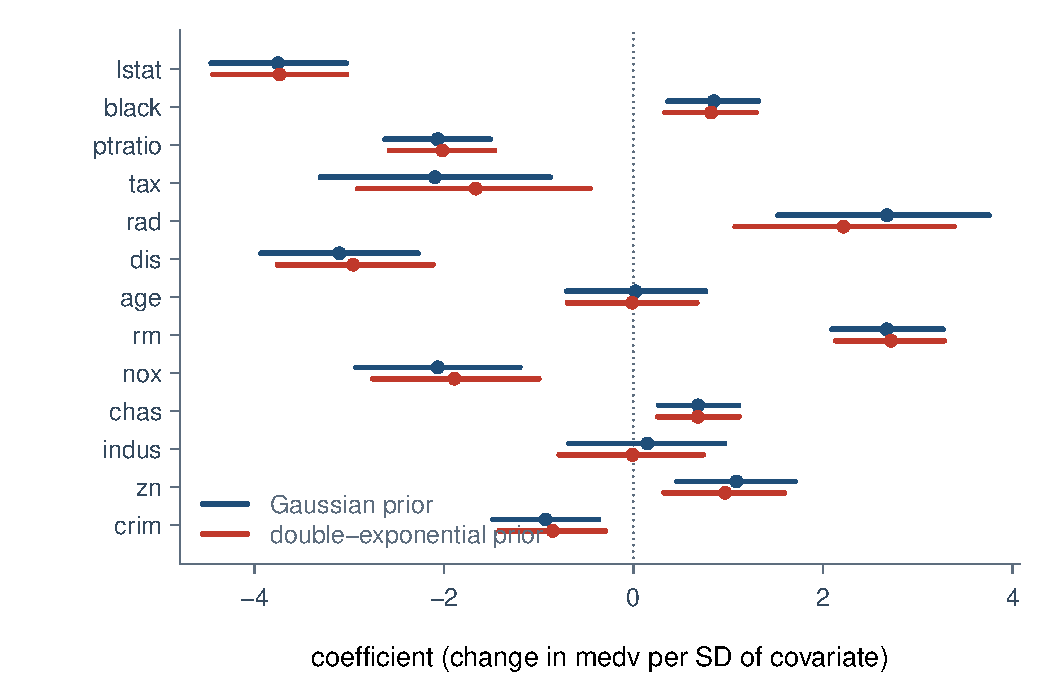
\includegraphics[width=0.8\linewidth]{ex02_coefficients.pdf}\end{center}
Posterior means change most for the weak or correlated covariates: \texttt{indus} $0.15\to-0.01$, \texttt{age} $0.02\to-0.01$ (both shrunk to $\approx0$), \texttt{rad} $2.67\to2.22$ and \texttt{tax} $-2.09\to-1.67$ (these two are highly correlated, $r=0.91$, so the prior pulls both toward 0). Strong effects (\texttt{lstat}, \texttt{rm}, \texttt{ptratio}) barely move. The posterior of $\lambda$ has mean 2.97, a mild amount of shrinkage --- with $n=506$ and $p=13$ the data dominate.

\step{(d) Prediction of rows 501--506.}
Fit on rows 1--500; for each posterior draw compute $\mathbf X_i\bm\beta^{(s)}+\sigma^{(s)}\varepsilon^{(s)}$.
\begin{center}
\begin{tabular}{ccccc}\toprule
Row & Actual & PPD mean & 95\% prediction interval & Inside?\\\midrule
501 & 16.8 & 20.7 & (11.3, 29.9) & yes\\
502 & 22.4 & 24.0 & (14.8, 33.5) & yes\\
503 & 20.6 & 22.9 & (13.5, 32.4) & yes\\
504 & 23.9 & 28.2 & (18.8, 37.9) & yes\\
505 & 22.0 & 26.6 & (17.2, 35.9) & yes\\
506 & 11.9 & 22.8 & (13.5, 32.3) & \textbf{no}\\\bottomrule
\end{tabular}
\end{center}
\begin{center}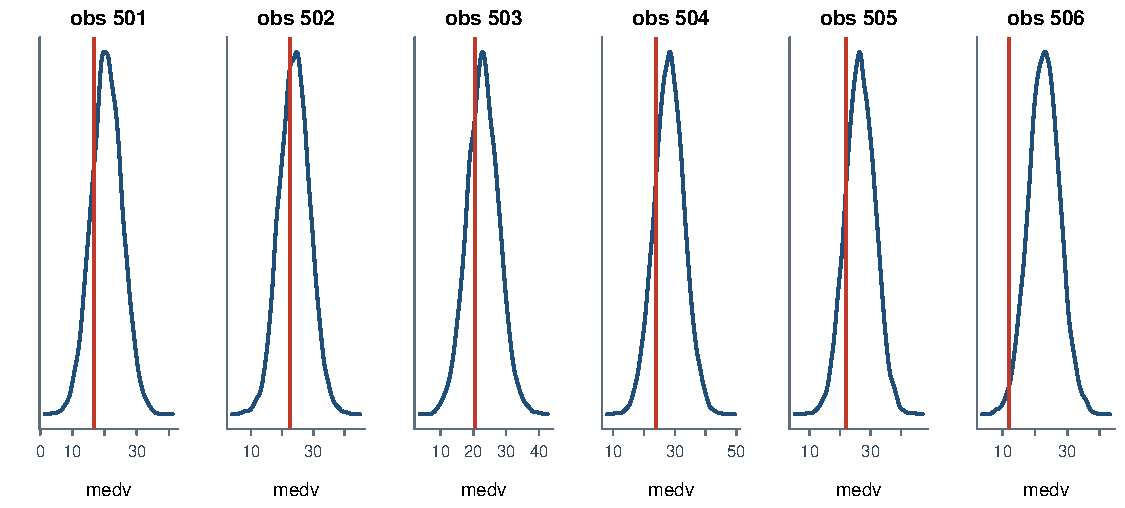
\includegraphics[width=0.98\linewidth]{ex02_ppd.pdf}\end{center}
Five of six actual values (red lines) fall inside their 95\% intervals, which is reasonable, but \emph{all six predictions are too high}. The last rows come from the same neighbourhood (the data are ordered by town), so they share an unmodelled local effect --- the errors are not independent.

\begin{answer}
(a) The sampler mixes essentially perfectly (ESS $\approx$ number of draws); see table. (b) Vague-prior Bayes $\approx$ least squares numerically; interpretation differs (probability statements about $\bm\beta$). (c) The LASSO prior shrinks weak/collinear coefficients (\texttt{indus}, \texttt{age}, \texttt{rad}, \texttt{tax}) toward 0 and leaves strong ones alone. (d) 5 of 6 held-out values are inside their 95\% PPD intervals, but all are over-predicted --- a sign of spatial correlation.
\end{answer}

\begin{takeaway}
A flat-prior Bayesian regression is ``least squares with uncertainty for free''; shrinkage priors matter most when covariates are many or highly correlated.
\end{takeaway}

% ================================================================= Exercise 3
\exercise{4.3 --- What explains the 2016 swing toward the Republican candidate?}

\begin{problem}{3}
Download the 2016 Presidential Election data from the book's website. Perform Bayesian linear regression with the response variable for county $i$ being the difference between the percentage of the vote for the Republican candidate in 2016 minus 2012 and all variables in the object X as covariates.
\begin{enumerate}[(a)]
\item Fit a Bayesian linear regression model with uninformative Gaussian priors for the regression coefficients, and summarize the posterior distribution of all regression coefficients.
\item Compute the residuals $R_i=Y_i-\mathbf X_i\hat{\bm\beta}$ where $\hat{\bm\beta}$ is the posterior mean of the regression coefficients. Are the residuals Gaussian? Which counties have the largest and smallest residuals, and what might this say about these counties?
\item Include a random effect for the state, that is, for a county in state $l=1,\dots,50$,
\[
Y_i\mid\alpha_l\sim\dist{Normal}(\mathbf X_i\bm\beta+\alpha_l,\sigma^2)
\]
where $\alpha_l\iid\dist{Normal}(0,\tau^2)$ and $\tau^2$ has an uninformative prior. Why might adding random effects be necessary? How does adding random effects affect the posterior of the regression coefficients? Which states have the highest and lowest posterior mean random effect, and what might this imply about these states?
\end{enumerate}
\end{problem}

\begin{restate}
Explain the county-level change in Republican vote share (2012 $\to$ 2016) with 10 demographic covariates, look at what the model misses, and add state effects.
\end{restate}

\begin{recall}
\begin{itemize}
\item Linear regression Gibbs sampler: primer, point 1. Random effects and hierarchical centring: primer, point 4.
\item A normal distribution has skewness 0 and excess kurtosis 0; a QQ plot of normal data is a straight line.
\end{itemize}
\end{recall}

\begin{keyidea}
Counties in the same state share candidates, campaigns and local politics, so their residuals are correlated. A state random effect absorbs this shared component.
\end{keyidea}

\solution
\step{Data.} $Y_i=100\times(\text{GOP share 2016}-\text{GOP share 2012})$ in percentage points, for 3{,}111 counties (32 counties without valid results dropped). Covariates (standardised): population change, \% aged 65+, \% Black, \% Hispanic, \% high-school graduates, \% bachelor's degree, home-ownership rate, median home value, median household income, \% in poverty.

\step{(a) Posterior summary} (Gaussian $\dist N(0,100^2)$ priors; coefficients per 1 SD of the covariate):
\begin{center}
\small
\begin{tabular}{lcccc}\toprule
Covariate & Mean & SD & 95\% interval & ESS (of 5000)\\\midrule
intercept & 3.838 & 0.071 & (3.70, 3.98) & 4992\\
population change 2010--14 & $-0.571$ & 0.086 & $(-0.74,-0.40)$ & 5000\\
\% aged 65+ & 0.826 & 0.105 & (0.62, 1.03) & 4812\\
\% Black & $-1.244$ & 0.087 & $(-1.42,-1.07)$ & 5000\\
\% Hispanic & $-1.666$ & 0.091 & $(-1.84,-1.49)$ & 4964\\
\% high-school graduates & 0.041 & 0.133 & $(-0.22, 0.30)$ & 5000\\
\% bachelor's degree & $\mathbf{-3.104}$ & 0.137 & $(-3.37,-2.83)$ & 4905\\
home-ownership rate & $-0.380$ & 0.105 & $(-0.59,-0.17)$ & 4864\\
median home value & $-0.581$ & 0.122 & $(-0.83,-0.34)$ & 4942\\
median household income & 1.031 & 0.198 & (0.64, 1.42) & 4711\\
\% in poverty & 0.370 & 0.152 & (0.07, 0.67) & 4874\\\bottomrule
\end{tabular}
\end{center}
The average county swung 3.8 points toward the Republican candidate. By far the strongest predictor is education: one SD more college graduates means a 3.1-point \emph{smaller} swing. Counties with more Black or Hispanic residents and faster-growing populations also swung less; older counties swung more.

\step{(b) Are the residuals Gaussian?}
\begin{center}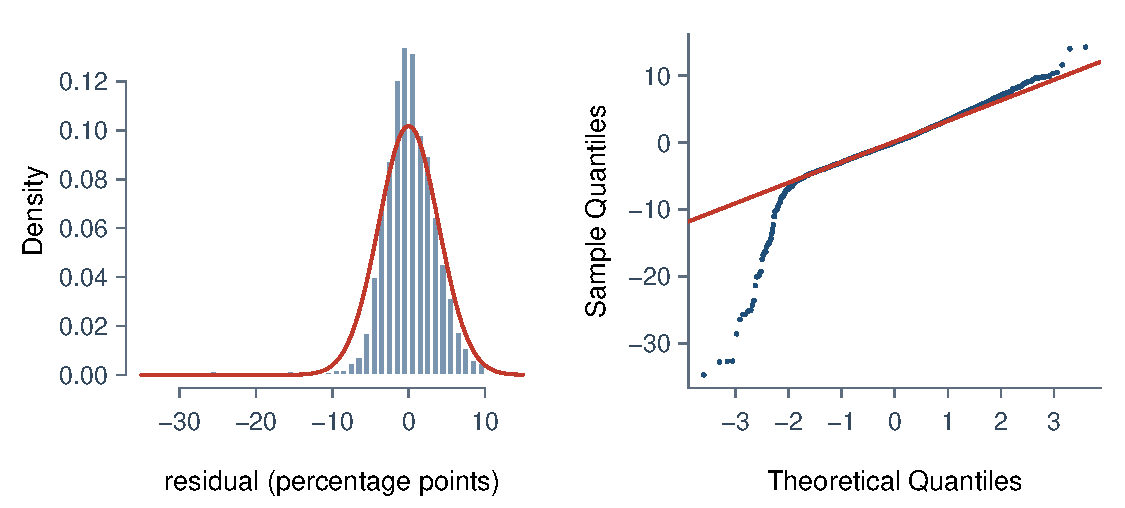
\includegraphics[width=0.9\linewidth]{ex03_residuals.pdf}\end{center}
\textbf{No.} Skewness $-1.92$ and excess kurtosis $13.0$: a long left tail. The QQ plot bends sharply at the lower end.
\begin{center}
\small
\begin{tabular}{lr|lr}\toprule
Most negative residuals & & Most positive residuals & \\\midrule
Madison County, ID & $-34.7$ & Elliott County, KY & 14.2\\
Utah County, UT & $-32.8$ & McKenzie County, ND & 14.0\\
Cache County, UT & $-32.7$ & Clark County, MO & 11.6\\
Davis County, UT & $-32.6$ & Howard County, IA & 10.5\\
Box Elder County, UT & $-28.6$ & Starr County, TX & 10.3\\\bottomrule
\end{tabular}
\end{center}
\emph{Interpretation.} The big negative residuals are heavily Latter-day Saint (Mormon) counties in Utah and Idaho, which strongly supported Mitt Romney (a Latter-day Saint) in 2012 and gave many votes to the independent Evan McMullin in 2016 --- something no demographic covariate in X captures. The positive residuals are rural, often traditionally Democratic counties (Elliott County, KY had never voted Republican before 2016) and the Hispanic border county Starr, TX, which swung unusually far toward the Republican candidate.

\step{(c) Why random effects?} Residuals cluster by state (state-average residuals range from $-19.1$ in Utah to $+9.7$ in DC), so counties in a state are \emph{not} independent: home-state candidates, state-wide campaigns and third-party candidates affect all counties in a state. Ignoring this treats 3{,}111 correlated counties as independent pieces of information and overstates precision.

\step{(c) Model.} $Y_i=\mathbf X_i\bm\beta+\alpha_{s_i}+\varepsilon_i$, $\alpha_l\iid\dist N(\mu,\tau^2)$ (with $\mu$ playing the role of the intercept), $\tau^2,\sigma^2\sim\dist{InvGamma}(0.01,0.01)$. Gibbs updates: $\bm\beta$ (normal), each $\alpha_l$ (normal, with precision $n_l/\sigma^2+1/\tau^2$), $\mu$ (normal), $\sigma^2,\tau^2$ (inverse-gamma). ESS for the 51 state effects: 3{,}023--5{,}000 out of 5{,}000.

\step{(c) Effect on the coefficients.}
\begin{center}
\small
\begin{tabular}{lcc|cc}\toprule
 & \multicolumn{2}{c|}{No random effects} & \multicolumn{2}{c}{State random effects}\\
Covariate & mean & SD & mean & SD\\\midrule
intercept / $\mu$ & 3.84 & 0.07 & 3.75 & 0.48\\
population change & $-0.57$ & 0.09 & $-0.25$ & 0.07\\
\% aged 65+ & 0.83 & 0.11 & 0.52 & 0.08\\
\% Black & $-1.24$ & 0.09 & $-0.85$ & 0.08\\
\% Hispanic & $-1.67$ & 0.09 & $-0.64$ & 0.09\\
\% high school & 0.04 & 0.13 & 0.44 & 0.11\\
\% bachelor's & $-3.10$ & 0.14 & $-3.25$ & 0.11\\
home ownership & $-0.38$ & 0.11 & 0.07 & 0.08\\
home value & $-0.58$ & 0.12 & 0.26 & 0.11\\
income & 1.03 & 0.20 & $-0.24$ & 0.15\\
poverty & 0.37 & 0.15 & 0.35 & 0.11\\\bottomrule
\end{tabular}
\end{center}
Residual SD drops from $\sigma=3.92$ to $2.70$; between-state SD $\tau\approx4.0$. Several coefficients shrink or even change sign (Hispanic $-1.67\to-0.64$, income $1.03\to-0.24$, home value $-0.58\to+0.26$): part of their apparent effect was really a \emph{state} effect (e.g.\ Utah counties have high incomes and home values). The education effect is robust. The uncertainty about the overall mean grows (SD 0.07 $\to$ 0.48) because there are effectively only 51 independent states for estimating it.

\step{(c) State effects.}
\begin{center}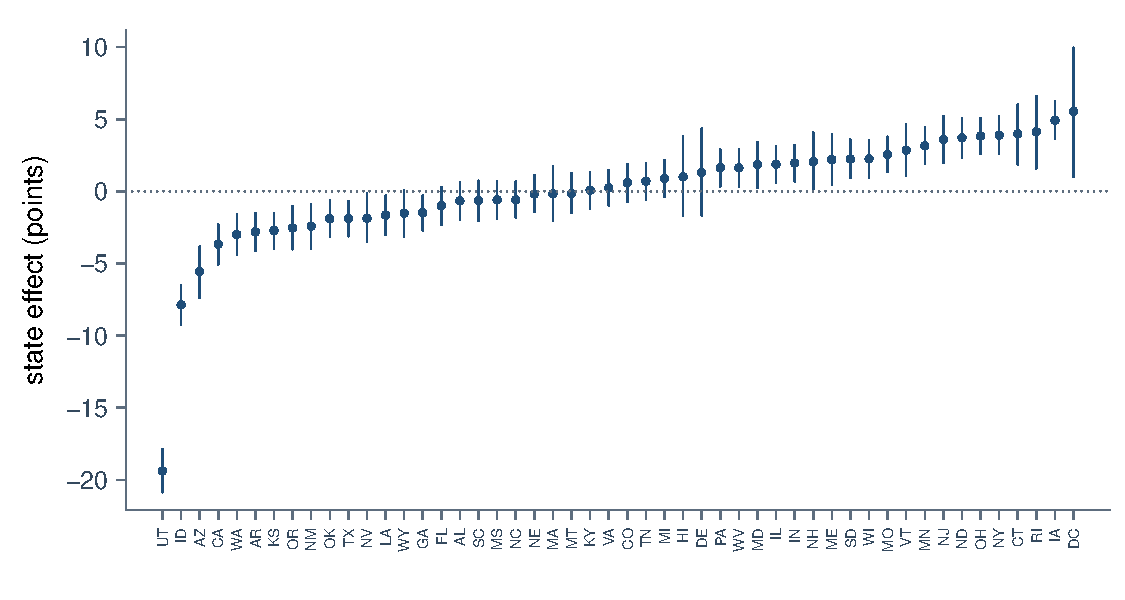
\includegraphics[width=0.98\linewidth]{ex03_state_effects.pdf}\end{center}
Lowest: Utah ($-19.4$), Idaho ($-7.9$), Arizona ($-5.6$), California ($-3.7$), Washington ($-3.0$). Highest: DC ($+5.6$), Iowa ($+4.9$), Rhode Island, Connecticut, New York ($\approx+4$). Interpretation: the Mountain West (large Latter-day Saint populations) and the West Coast swung less toward the Republican candidate than their demographics predict, while Iowa and parts of the North-East swung more --- consistent with the regional story of the 2016 election.

\begin{answer}
(a) Education (\% bachelor's) is the dominant predictor (one SD $\Rightarrow-3.1$ points); see table. (b) Residuals are clearly non-Gaussian (heavy left tail); the worst-fitted counties are Latter-day Saint counties in Utah/Idaho (negative) and rural KY/ND/MO/IA and Starr County TX (positive). (c) State effects are needed because counties within a state are correlated; they reduce $\sigma$ from 3.9 to 2.7, change several coefficients, and identify Utah/Idaho (lowest) and Iowa/North-East (highest).
\end{answer}

\begin{takeaway}
Large residuals are often the most interesting part of a regression: they point to variables the model is missing (here, religion and regional politics).
\end{takeaway}

% ================================================================= Exercise 4
\exercise{4.4 --- Gun laws and homicides}

\begin{problem}{4}
Download the US gun control data from the book's website. These data are taken from the cross-sectional study in [86]. For state $i$, let $Y_i$ be the number of homicides and $N_i$ be the population.
\begin{enumerate}[(a)]
\item Fit the model $Y_i|\bm\beta\sim\dist{Poisson}(N_i\lambda_i)$ where $\log(\lambda_i)=\mathbf X_i\bm\beta$. Use uninformative priors and $p=7$ covariates in $\mathbf X_i$: the intercept, the five confounders $Z_i$, and the total number of gun laws in state $i$. Provide justification that the MCMC sampler has converged and sufficiently explored the posterior distribution and summarize the posterior of $\bm\beta$.
\item Fit a negative binomial regression model, and compare with the results from Poisson regression.
\item For the Poisson model in (a), compute the posterior predictive distribution for each state with the number of gun laws set to zero. Repeat this with the number of gun laws set to 25 (the maximum number). According to these calculations, how would the number of deaths nationwide be affected by these policy changes? Do you trust these projections?
\end{enumerate}
\end{problem}

\begin{restate}
Model state death counts with a Poisson regression on five confounders and the number of gun laws; check for over-dispersion with a negative binomial; then predict national deaths under ``no laws'' and ``all 25 laws''.
\end{restate}

\begin{recall}
\begin{itemize}
\item Poisson regression with offset: $\log\E(Y_i)=\log N_i+\mathbf X_i\bm\beta$; $e^{\beta_j}$ is a rate ratio (primer, point 3).
\item \textbf{Negative binomial}: $Y\sim\dist{NB}(\text{mean }\mu,\text{size }r)$ has $\V(Y)=\mu+\mu^2/r$ $>$ mean. As $r\to\infty$ it becomes Poisson. It allows extra-Poisson variation (over-dispersion).
\end{itemize}
\end{recall}

\begin{keyidea}
Use block Metropolis with the GLM covariance as proposal. Check convergence with three chains ($\hat R$, ESS). For the projections, simulate every state's count under the new law count and add them up --- one national total per posterior draw.
\end{keyidea}

\solution
\step{Data and covariates.} 50 states. Confounders $Z$: 2009 firearm death rate, firearm-ownership quartile, unemployment quartile, non-firearm homicide quartile, firearm-export quartile. Laws: number of the 25 laws each state has (mean 5.1, SD 5.6, range 0--21). All covariates standardised; priors $\beta_j\sim\dist N(0,10^2)$.

\step{(a) Convergence.} Three chains $\times$ 20{,}000 kept iterations, acceptance 27--28\% (close to the optimal 23--30\% for 7 parameters); every $\hat R\le1.002$ and ESS $\approx2{,}500$ per coefficient --- converged and well explored.
\begin{center}
\small
\begin{tabular}{lcccc}\toprule
Coefficient (per SD) & Mean & SD & 95\% interval & $\hat R$\\\midrule
intercept & $-9.165$ & 0.007 & $(-9.179,-9.151)$ & 1.000\\
2009 rate & 0.324 & 0.015 & (0.295, 0.352) & 1.001\\
ownership & $-0.047$ & 0.011 & $(-0.068,-0.026)$ & 1.001\\
unemployment & 0.018 & 0.007 & (0.004, 0.032) & 1.002\\
non-firearm homicide & $-0.006$ & 0.010 & $(-0.026, 0.014)$ & 1.002\\
export & 0.000 & 0.007 & $(-0.014, 0.014)$ & 1.001\\
\textbf{laws} & $\mathbf{-0.078}$ & 0.008 & $(-0.094,-0.062)$ & 1.000\\\bottomrule
\end{tabular}
\end{center}
Per extra law (divide by the SD 5.61): rate ratio $e^{-0.078/5.61}=0.986$, i.e.\ \textbf{1.4\% fewer deaths per law} (95\% CI 1.1--1.7\%).

\step{(b) Negative binomial.}
The Poisson fit is over-dispersed: Pearson $\chi^2/\text{df}=2.70$ (should be $\approx1$). Adding a size parameter $r$ (prior $\dist{Gamma}(0.1,0.1)$, sampled as $\log r$):
\begin{center}
\small
\begin{tabular}{lcc|ccc}\toprule
 & \multicolumn{2}{c|}{Poisson} & \multicolumn{3}{c}{Negative binomial}\\
Coefficient & mean & SD & mean & SD & 95\% interval\\\midrule
2009 rate & 0.324 & 0.015 & 0.307 & 0.038 & (0.232, 0.382)\\
ownership & $-0.047$ & 0.011 & $-0.045$ & 0.026 & $(-0.097, 0.007)$\\
unemployment & 0.018 & 0.007 & 0.009 & 0.021 & $(-0.033, 0.051)$\\
laws & $-0.078$ & 0.008 & $-0.099$ & 0.026 & $(-0.151,-0.048)$\\\bottomrule
\end{tabular}
\end{center}
The point estimates are similar, but every SD is 2.5--3 times larger: the Poisson model was over-confident. Ownership and unemployment are no longer clearly non-zero. $r\approx88$ (mild but real over-dispersion). The laws effect remains negative with a much wider interval.

\step{(c) National projections} (Poisson model, 20{,}000 posterior draws; each state simulated with its own confounders):
\begin{center}
\begin{tabular}{lcc}\toprule
Scenario & PPD mean of national total & 95\% prediction interval\\\midrule
Current laws (check) & 31{,}570 & --- \quad(observed 31{,}573)\\
0 laws in every state & 34{,}477 & (33{,}656, 35{,}302)\\
25 laws in every state & 24{,}350 & (22{,}999, 25{,}741)\\\bottomrule
\end{tabular}
\end{center}
\begin{center}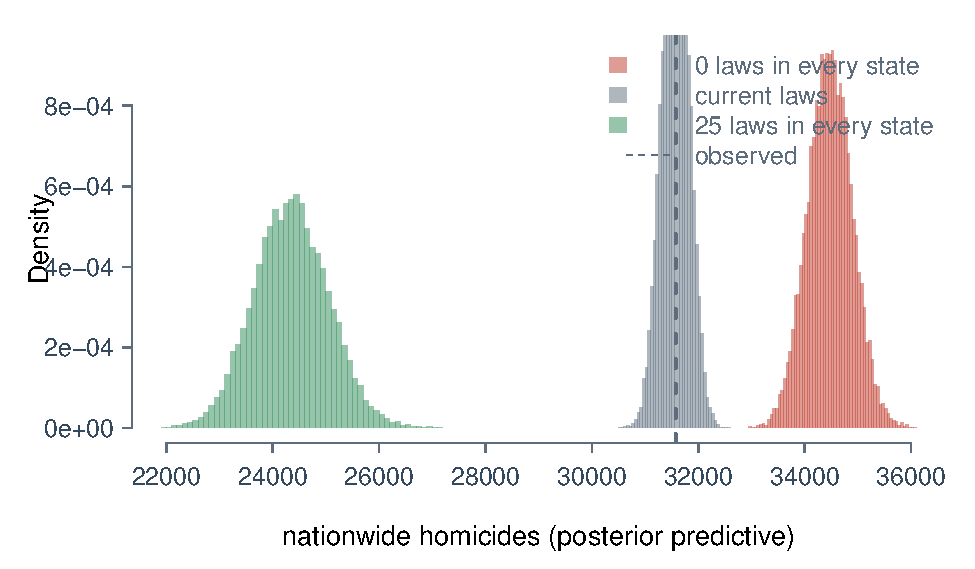
\includegraphics[width=0.72\linewidth]{ex04_ppd.pdf}\end{center}
Taken literally: repealing all laws would add $\approx2{,}900$ deaths a year, adopting all 25 would prevent $\approx7{,}200$.

\step{(c) Do we trust these projections? No:}
\begin{itemize}
\item \textbf{Observational, cross-sectional data}: states with many laws differ in countless unmeasured ways; the coefficient is an association, not a causal effect.
\item \textbf{Extrapolation}: no state has more than 21 laws, so ``25 laws everywhere'' is outside the data.
\item \textbf{Over-dispersion}: the Poisson intervals are far too narrow (part b).
\item Counting laws assumes every law has the same effect and that effects add up on the log scale.
\end{itemize}

\begin{sanity}
The Poisson PPD under the \emph{current} laws reproduces the observed national total (31{,}570 vs.\ 31{,}573), so the simulation machinery is correct. \checkmark
\end{sanity}

\begin{answer}
(a) Converged ($\hat R\le1.002$, ESS $\approx2{,}500$); each extra law is associated with 1.4\% fewer deaths. (b) The NB model fits the over-dispersion ($r\approx88$); estimates similar, SDs 2.5--3$\times$ larger. (c) $\approx34{,}500$ deaths with 0 laws and $\approx24{,}400$ with 25 laws vs.\ 31{,}600 now --- but these projections are not trustworthy (confounding, extrapolation, over-confident Poisson intervals).
\end{answer}

\begin{takeaway}
A beautifully converged MCMC sampler says nothing about whether the model answers a causal question.
\end{takeaway}

% ================================================================= Exercise 5
\exercise{4.5 --- Who survived the Titanic?}

\begin{problem}{5}
Download the titanic dataset from R,
\begin{lstlisting}
library("titanic")
dat <- titanic_train
?titanic_train
\end{lstlisting}
Let $Y_i=1$ if passenger $i$ survived and $Y_i=0$ otherwise. Perform a Bayesian logistic regression of the survival probability onto the passenger's age, gender (dummy variable) and class (two dummy variables). Summarize the effect of each covariate.
\end{problem}

\begin{restate}
Model the probability of surviving the Titanic as a function of age, sex and ticket class.
\end{restate}

\begin{recall}
Logistic regression: $\log\frac{p_i}{1-p_i}=\mathbf X_i\bm\beta$. Log-likelihood $\sum_i\{Y_i\eta_i-\log(1+e^{\eta_i})\}$ with $\eta_i=\mathbf X_i\bm\beta$. $e^{\beta_j}$ is the \textbf{odds ratio} for a one-unit change in $X_j$; probabilities come from $p=\frac{e^\eta}{1+e^\eta}$.
\end{recall}

\begin{keyidea}
Dummy coding: \texttt{female} = 1 for women; \texttt{class2}, \texttt{class3} = 1 for 2nd/3rd class (1st class is the baseline). Age is centred at 30 and measured in decades.
\end{keyidea}

\solution
\step{Data.} 891 passengers; 177 have missing age, leaving \textbf{714 complete cases} (survival rate 40.6\%). (Dropping incomplete cases assumes age is missing at random; imputing age inside the MCMC would be the fuller Bayesian approach.)
\step{Model.} $\mathrm{logit}\,p_i=\beta_0+\beta_1\frac{\text{age}_i-30}{10}+\beta_2\,\text{female}_i+\beta_3\,\text{class2}_i+\beta_4\,\text{class3}_i$, $\beta_j\sim\dist N(0,10^2)$. Block Metropolis, three chains $\times$ 16{,}000 kept draws, acceptance 28\%, all $\hat R\le1.002$.
\begin{center}
\small
\begin{tabular}{lcccc|c}\toprule
 & Mean & 95\% interval & Odds ratio & OR 95\% interval & GLM\\\midrule
intercept & 0.140 & $(-0.26, 0.54)$ & --- & --- & 0.145\\
age (per 10 yr) & $-0.373$ & $(-0.53,-0.23)$ & 0.689 & (0.59, 0.80) & $-0.370$\\
female & 2.541 & (2.14, 2.95) & \textbf{12.7} & (8.5, 19.1) & 2.523\\
2nd class & $-1.313$ & $(-1.85,-0.76)$ & 0.269 & (0.16, 0.47) & $-1.310$\\
3rd class & $-2.596$ & $(-3.15,-2.04)$ & 0.075 & (0.04, 0.13) & $-2.581$\\\bottomrule
\end{tabular}
\end{center}
\step{Turning odds into probabilities} (30-year-old passenger; posterior median and 95\% interval):
\begin{center}
\begin{tabular}{lcc}\toprule
 & Man & Woman\\\midrule
1st class & 0.54 (0.44, 0.63) & 0.94 (0.90, 0.96)\\
2nd class & 0.24 (0.17, 0.31) & 0.80 (0.72, 0.86)\\
3rd class & 0.08 (0.06, 0.11) & 0.52 (0.43, 0.61)\\\bottomrule
\end{tabular}
\end{center}
\why{For a 30-year-old man in 1st class, $\eta=\beta_0$, so $p=\frac{e^{0.14}}{1+e^{0.14}}=0.535$; a woman adds $\beta_2=2.54$: $p=\frac{e^{2.68}}{1+e^{2.68}}=0.936$.}

\begin{answer}
\textbf{Sex}: women had about 12.7 times the odds of survival of men (``women and children first''). \textbf{Class}: compared with 1st class, the odds were 73\% lower in 2nd class (OR 0.27) and 92\% lower in 3rd class (OR 0.075). \textbf{Age}: each extra decade reduced the odds by about 31\% (OR 0.69). All effects are clearly non-zero.
\end{answer}

\begin{takeaway}
Report odds ratios \emph{and} a few predicted probabilities --- probabilities are much easier to communicate (94\% for a first-class woman vs.\ 8\% for a third-class man).
\end{takeaway}

% ================================================================= Exercise 6
\exercise{4.6 --- A gamma regression for \emph{T.\ rex} growth}

\begin{problem}{6}
The T. rex growth chart data plotted in Figure 3.10 has $n=6$ observations with weights (kg) 29.9, 1761, 1807, 2984, 3230, 5040, and 5654 and corresponding ages (years) 2, 15, 14, 16, 18, 22 and 28. Since weight must be positive, the gamma family of distributions is a reasonable model for these data. Describe a model with gamma likelihood and log mean that increases linearly with age. Approximate the posterior using MCMC, summarize the posterior distribution of all model parameters, and plot the data versus the fitted mean curve.
\end{problem}

\begin{restate}
Model positive body masses with a gamma distribution whose (log) mean grows linearly with age, fit it by MCMC and draw the fitted growth curve.
\end{restate}

\begin{recall}
\textbf{Gamma regression (mean--shape form).} $Y_i\sim\dist{Gamma}(\nu,\ \nu/\mu_i)$ (shape $\nu$, rate $\nu/\mu_i$) has mean $\mu_i$ and variance $\mu_i^2/\nu$: the SD is proportional to the mean, natural for positive data. With $\log\mu_i=\beta_0+\beta_1\,\text{age}_i$, $e^{\beta_1}$ is the multiplicative change in mean mass per year.
\end{recall}

\begin{keyidea}
Three unknowns $(\beta_0,\beta_1,\nu)$; sample $(\beta_0,\beta_1,\log\nu)$ jointly by random-walk Metropolis (log scale keeps $\nu>0$; remember the Jacobian $+\log\nu$).
\end{keyidea}

\solution
\step{Note on the data.} The exercise says $n=6$ but lists 7 (mass, age) pairs (the same 7 as Listing 3.9); we use all 7.
\step{Model.}
\[
\text{mass}_i\sim\dist{Gamma}\big(\nu,\ \nu/\mu_i\big),\quad\log\mu_i=\beta_0+\beta_1\,\text{age}_i,\quad\beta_0,\beta_1\sim\dist N(0,10^2),\quad\nu\sim\dist{Gamma}(0.1,0.1).
\]
\step{MCMC.} Three chains $\times$ 50{,}000 kept draws; acceptance 49\%; $\hat R\le1.002$ for all parameters.
\begin{center}
\begin{tabular}{lccc}\toprule
 & Mean & SD & 95\% interval\\\midrule
$\beta_0$ & 4.40 & 1.11 & (2.41, 6.84)\\
$\beta_1$ & 0.199 & 0.064 & (0.066, 0.323)\\
$\nu$ (shape) & 1.98 & 1.08 & (0.50, 4.63)\\
growth per year $100(e^{\beta_1}-1)$ & 22.2\% & 7.9\% & (6.8\%, 38.1\%)\\\bottomrule
\end{tabular}
\end{center}
\begin{center}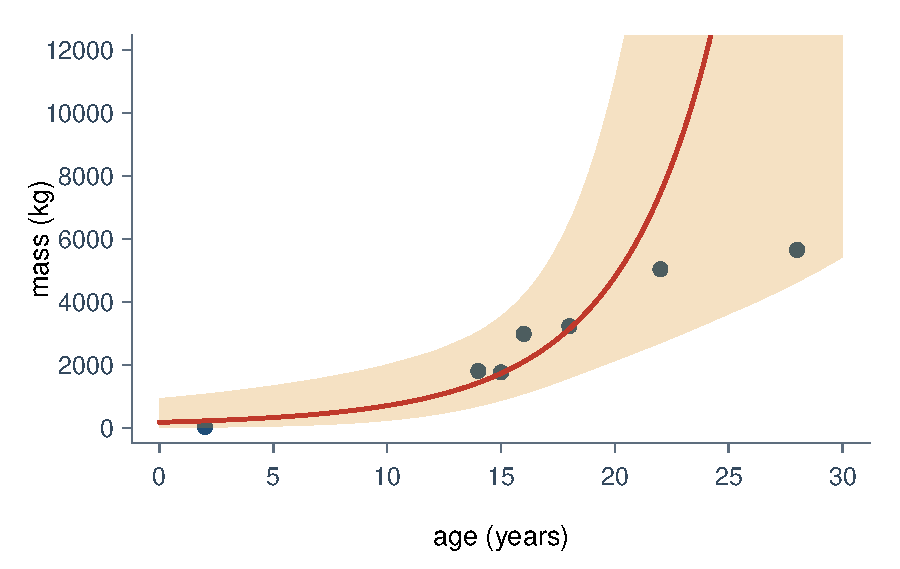
\includegraphics[width=0.66\linewidth]{ex06_fit.pdf}\end{center}
\step{Interpretation.} Mean mass grows by about 22\% per year. A small shape ($\nu\approx2$) means a large coefficient of variation ($1/\sqrt\nu\approx0.7$), driven by the age-2 juvenile (29.9 kg) which the exponential curve over-predicts. The wide band shows how little 7 fossils can tell us.

\begin{sanity}
The classical gamma GLM gives $\hat\beta_0=4.30$, $\hat\beta_1=0.199$: the same slope. \checkmark
\end{sanity}

\begin{answer}
Model: $\text{mass}_i\sim\dist{Gamma}(\nu,\nu/\mu_i)$, $\log\mu_i=\beta_0+\beta_1\text{age}_i$. Posterior: $\beta_1\approx0.20$ (95\% CI 0.07--0.32), i.e.\ $\approx22\%$ growth per year; $\nu\approx2$. The fitted curve follows the data but with wide uncertainty.
\end{answer}

\begin{takeaway}
An exponential growth curve cannot level off; real dinosaur growth is sigmoidal. Compare the power-law curve in Exercise 3.17 --- with 7 points, several shapes fit about equally well.
\end{takeaway}

% ================================================================= Exercise 7
\exercise{4.7 --- Gibbs sampler for the one-way random effects model}

\begin{problem}{7}
Consider the one-way random effects model $Y_{ij}|\alpha_i,\sigma^2\sim\dist{Normal}(\alpha_i,\sigma^2)$ and $\alpha_i\sim\dist{Normal}(0,\tau^2)$ for $i=1,\dots,n$ and $j=1,\dots,m$. Assuming conjugate priors $\sigma^2,\tau^2\sim\dist{InvGamma}(a,b)$, derive the full conditional distributions of $\alpha_1$, $\sigma^2$ and $\tau^2$, and outline (but do not code) an MCMC algorithm to sample from the posterior.
\end{problem}

\begin{restate}
$n$ groups, $m$ observations each; each group has its own mean $\alpha_i$, drawn from a common normal. Derive the three Gibbs updates and write the algorithm.
\end{restate}

\begin{recall}
Completing the square: a log density $-\frac A2x^2+Bx$ means $x\sim\dist N(B/A,1/A)$. Inverse-gamma kernel: $x^{-a-1}e^{-b/x}$.
\end{recall}

\begin{keyidea}
Write the joint posterior once, then for each parameter keep only the factors that contain it.
\end{keyidea}

\solution
\step{Joint posterior.}
\[
p(\bm\alpha,\sigma^2,\tau^2\mid\mathbf Y)\propto\prod_{i=1}^n\prod_{j=1}^m(\sigma^2)^{-\frac12}e^{-\frac{(Y_{ij}-\alpha_i)^2}{2\sigma^2}}\ \prod_{i=1}^n(\tau^2)^{-\frac12}e^{-\frac{\alpha_i^2}{2\tau^2}}\ (\sigma^2)^{-a-1}e^{-\frac b{\sigma^2}}\ (\tau^2)^{-a-1}e^{-\frac b{\tau^2}}.
\]
\step{Full conditional of $\alpha_1$.} Factors with $\alpha_1$: $-\frac{1}{2\sigma^2}\sum_j(Y_{1j}-\alpha_1)^2-\frac{\alpha_1^2}{2\tau^2}$. Coefficient of $\alpha_1^2$: $A=\frac m{\sigma^2}+\frac1{\tau^2}$; coefficient of $\alpha_1$: $B=\frac{\sum_jY_{1j}}{\sigma^2}=\frac{m\bar Y_1}{\sigma^2}$. So
\[
\alpha_1\mid\cdot\ \sim\ \dist N\Big(\frac{m\bar Y_1/\sigma^2}{m/\sigma^2+1/\tau^2},\ \frac{1}{m/\sigma^2+1/\tau^2}\Big).
\]
\why{The mean is a precision-weighted compromise between the group average $\bar Y_1$ and the prior mean 0: groups are shrunk toward 0 more when $\tau^2$ is small or $m$ is small.}
\step{Full conditional of $\sigma^2$.} Collect all $nm$ likelihood terms and the prior:
\[
p(\sigma^2\mid\cdot)\propto(\sigma^2)^{-\frac{nm}2-a-1}\exp\Big\{-\frac{b+\frac12\sum_{i,j}(Y_{ij}-\alpha_i)^2}{\sigma^2}\Big\},
\]
so
\[
\sigma^2\mid\cdot\sim\dist{InvGamma}\Big(a+\frac{nm}{2},\ b+\frac12\sum_{i,j}(Y_{ij}-\alpha_i)^2\Big).
\]
\step{Full conditional of $\tau^2$.} Only the $n$ random-effect terms and its prior:
\[
\tau^2\mid\cdot\sim\dist{InvGamma}\Big(a+\frac n2,\ b+\frac12\sum_{i=1}^n\alpha_i^2\Big).
\]
\step{Algorithm.}
\begin{enumerate}[1.]
\item Initialise $\alpha_i^{(0)}=\bar Y_i$, $\sigma^{2(0)}=$ average within-group variance, $\tau^{2(0)}=$ variance of the $\bar Y_i$.
\item For $s=1,\dots,S$: (i) for $i=1,\dots,n$ draw $\alpha_i^{(s)}$ from its normal full conditional using $\sigma^{2(s-1)},\tau^{2(s-1)}$; (ii) draw $\sigma^{2(s)}$ given $\bm\alpha^{(s)}$; (iii) draw $\tau^{2(s)}$ given $\bm\alpha^{(s)}$.
\item Discard burn-in; check trace plots, $\hat R$ (several chains) and ESS --- particularly for $\tau^2$, which mixes slowest when $n$ is small.
\end{enumerate}

\begin{answer}
$\alpha_1\mid\cdot\sim\dist N\big(\frac{m\bar Y_1/\sigma^2}{m/\sigma^2+1/\tau^2},\frac1{m/\sigma^2+1/\tau^2}\big)$; $\sigma^2\mid\cdot\sim\dist{InvGamma}(a+\frac{nm}2,\ b+\frac12\sum_{ij}(Y_{ij}-\alpha_i)^2)$; $\tau^2\mid\cdot\sim\dist{InvGamma}(a+\frac n2,\ b+\frac12\sum_i\alpha_i^2)$. Cycle through them (Gibbs).
\end{answer}

\begin{takeaway}
This is exactly the sampler used (with covariates added) for the state effects in Exercise 3.
\end{takeaway}

% ================================================================= Exercise 8
\exercise{4.8 --- Malaria in Gambian children}

\begin{problem}{8}
Load the Gambia data in R:
\begin{lstlisting}
> library(geoR)
> data(gambia)
> ?gambia
\end{lstlisting}
The response variable $Y_i$ is the binary indicator that child $i$ tested positive for malaria (pos), and the remaining seven variables are covariates.
\begin{enumerate}[(a)]
\item Fit the logistic regression model
\[
\mathrm{logit}[\Prob(Y_i=1)]=\sum_{j=1}^pX_{ij}\beta_j
\]
with uninformative priors for the $\beta_j$. Verify that the MCMC sampler has converged, and summarize the effects of the covariates.
\item In this dataset, the 2,035 children reside in $L=65$ unique locations (defined by the x and y coordinates in the dataset). Let $s_i\in\{1,\dots,L\}$ be the label of the location for observation $i$. Fit the random effects logistic regression model
\[
\mathrm{logit}[\Prob(Y_i=1)]=\sum_{j=1}^pX_{ij}\beta_j+\alpha_{s_i}\quad\text{where}\quad\alpha_l\iid\dist{Normal}(0,\tau^2)
\]
and the $\beta_j$ and $\tau^2$ have uninformative priors. Verify that the MCMC sampler has converged; explain why random effects might be needed here; discuss and explain any differences in the posteriors of the regression coefficients that occur when random effects are added to the model; plot the posterior means of the $\alpha_l$ by their spatial locations, and suggest how this map might be useful to malaria researchers.
\end{enumerate}
\end{problem}

\begin{restate}
Model which children test positive for malaria using age, bed-net use, insecticide treatment, greenness, a health-centre indicator and the village coordinates; then add village effects and map them.
\end{restate}

\begin{recall}
\begin{itemize}
\item Logistic regression and block Metropolis: primer, point 3.
\item \textbf{Location-level covariates} (same value for every child in a village: \texttt{green}, \texttt{phc}, \texttt{x}, \texttt{y}) can only be learned from \emph{differences between villages}.
\end{itemize}
\end{recall}

\begin{keyidea}
Children in the same village share mosquitoes, water and health care, so their outcomes are correlated. Ignoring this pretends we have 2{,}035 independent pieces of information about village-level covariates when we really have 65.
\end{keyidea}

\solution
\step{Covariates} (continuous ones standardised): age (years), \texttt{netuse} (sleeps under a bed net), \texttt{treated} (net treated with insecticide), \texttt{green} (satellite greenness), \texttt{phc} (village has a primary health centre), and the coordinates \texttt{x}, \texttt{y}. Prevalence: 35.7\%.

\step{(a) Logistic regression.} Three chains $\times$ 12{,}000 kept draws, acceptance 27\%, all $\hat R\le1.002$.
\begin{center}
\small
\begin{tabular}{lccc|c}\toprule
 & Mean & SD & 95\% interval & Odds ratio\\\midrule
intercept & 0.161 & 0.114 & $(-0.06, 0.38)$ & ---\\
age (per SD) & 0.267 & 0.048 & (0.17, 0.36) & 1.31\\
netuse & $-0.697$ & 0.119 & $(-0.93,-0.46)$ & 0.50\\
treated & $-0.032$ & 0.140 & $(-0.32, 0.24)$ & 0.97\\
green (per SD) & $-0.029$ & 0.094 & $(-0.21, 0.16)$ & 0.97\\
phc & $-0.445$ & 0.117 & $(-0.67,-0.21)$ & 0.64\\
x (per SD) & 0.386 & 0.092 & (0.20, 0.56) & 1.47\\
y (per SD) & $-0.338$ & 0.053 & $(-0.44,-0.24)$ & 0.71\\\bottomrule
\end{tabular}
\end{center}
Older children are more likely to test positive; bed nets halve the odds; a health centre lowers the odds by a third; prevalence increases eastward and southward.

\step{(b) Why random effects?} Villages differ in many unmeasured ways (breeding sites, housing, distance to water). Children in one village therefore share a common risk: residuals are correlated within villages, and treating them as independent understates the uncertainty of village-level effects.

\step{(b) Model and sampler.} $\alpha_l\iid\dist N(\mu,\tau^2)$ (centred), $\tau^2\sim\dist{InvGamma}(0.1,0.1)$. Each iteration: a block Metropolis step for $\bm\beta$, a Metropolis step for all 65 $\alpha_l$ at once (they are conditionally independent given $\bm\beta$), Gibbs draws for $\mu$ and $\tau^2$. Three chains $\times$ 20{,}000 kept draws.

\step{(b) Convergence.} All $\hat R\le1.013$. ESS ranges from 230 (\texttt{phc}) to 1{,}700 (age), and 2{,}037 for $\tau$. The village-level coefficients mix more slowly because they trade off against the village effects --- precisely the confounding described above --- but the ESS is adequate for posterior means and 95\% intervals.

\step{(b) Effect on the coefficients.}
\begin{center}
\small
\begin{tabular}{lcc|ccc}\toprule
 & \multicolumn{2}{c|}{No random effects} & \multicolumn{3}{c}{Village random effects}\\
 & mean & SD & mean & SD & 95\% interval\\\midrule
age & 0.267 & 0.048 & 0.288 & 0.052 & (0.19, 0.39)\\
netuse & $-0.697$ & 0.119 & $-0.505$ & 0.160 & $(-0.82,-0.19)$\\
treated & $-0.032$ & 0.140 & $-0.274$ & 0.205 & $(-0.67, 0.13)$\\
green & $-0.029$ & 0.094 & $-0.098$ & 0.227 & $(-0.55, 0.36)$\\
phc & $-0.445$ & 0.117 & $-0.458$ & 0.232 & $(-0.92,-0.00)$\\
x & 0.386 & 0.092 & 0.503 & 0.229 & (0.05, 0.95)\\
y & $-0.338$ & 0.053 & $-0.365$ & 0.113 & $(-0.58,-0.14)$\\
$\tau$ & --- & --- & 0.795 & 0.106 & (0.61, 1.03)\\\bottomrule
\end{tabular}
\end{center}
\begin{itemize}
\item \textbf{Child-level} covariates (age) barely change.
\item \textbf{Village-level} covariates (\texttt{green}, \texttt{phc}, \texttt{x}, \texttt{y}): SDs roughly \emph{double} --- they are now (correctly) estimated from 65 villages rather than 2{,}035 children.
\item The bed-net effect shrinks ($-0.70\to-0.51$): part of the naive effect was villages with high net use also being low-risk villages.
\item $\tau\approx0.8$: substantial variation between villages (an odds ratio of $e^{2\times0.8}\approx5$ between a high-risk and a low-risk village two SDs apart).
\end{itemize}

\step{(b) Map of village effects.}
\begin{center}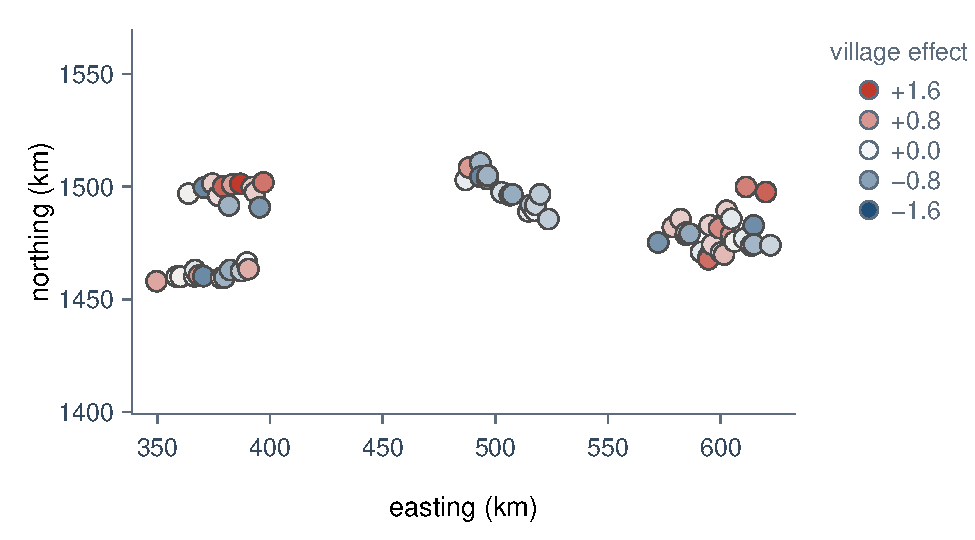
\includegraphics[width=0.8\linewidth]{ex08_map.pdf}\end{center}
Red villages have higher malaria risk than their covariates predict, blue ones lower (effects from $-1.05$ to $+1.58$ on the log-odds scale). Researchers can use this map to (i) target bed-net distribution and spraying at red ``hotspots'', (ii) look for environmental causes shared by neighbouring red villages (rice fields, river proximity), and (iii) design future surveys.

\begin{answer}
(a) Converged; age $+$, bed nets $-$ (OR 0.5), health centre $-$, east/south higher risk; insecticide treatment and greenness unclear. (b) Converged ($\hat R\le1.013$); random effects are needed because children within a village are correlated; adding them leaves child-level effects alone but roughly doubles the uncertainty of village-level effects and weakens the bed-net effect; $\tau\approx0.8$. The map highlights high-risk villages for targeted intervention.
\end{answer}

\begin{takeaway}
Whenever covariates are measured at a group level, a model without group effects is over-confident about them.
\end{takeaway}

% ================================================================= Exercise 9
\exercise{4.9 --- How popular will the name ``Sophia'' be?}

\begin{problem}{9}
Download the babynames data in R, and compute the log odds of a baby being named ``Sophia'' each year after 1950:
\begin{lstlisting}
library(babynames)
dat <- babynames
dat <- dat[dat$name=="Sophia" &
           dat$sex=="F" &
           dat$year>1950,]
yr <- dat$year
p  <- dat$prop
t  <- dat$year - 1950
Y  <- log(p/(1-p))
\end{lstlisting}
Let $Y_t$ denote the sample log-odds in year $t+1950$. Fit the following time series (auto-regressive order 1) model to these data:
\[
Y_t=\mu_t+\rho(Y_{t-1}-\mu_{t-1})+\varepsilon_t
\]
where $\mu_t=\alpha+\beta t$ and $\varepsilon_t\iid\dist{Normal}(0,\sigma^2)$. The priors are $\alpha,\beta\sim\dist{Normal}(0,100^2)$, $\rho\sim\dist{Uniform}(-1,1)$, and $\sigma^2\sim\dist{InvGamma}(0.1,0.1)$.
\begin{enumerate}[(a)]
\item Give an interpretation of each of the four model parameters: $\alpha$, $\beta$, $\rho$, and $\sigma^2$.
\item Fit the model using JAGS for $t>1$, verify convergence, and report the posterior mean and 95\% interval for each parameter.
\item Plot the posterior predictive distribution for $Y_t$ in the year 2020.
\end{enumerate}
\end{problem}

\begin{restate}
Model the year-by-year log-odds of the name Sophia as a linear trend plus persistent deviations, and forecast 2020.
\end{restate}

\begin{recall}
\begin{itemize}
\item \textbf{AR(1)}: $e_t=\rho e_{t-1}+\varepsilon_t$ with $|\rho|<1$ is stationary --- deviations decay back to 0. As $\rho\to1$ it becomes a \emph{random walk}, which never returns.
\item Given $\rho$, the model is linear in $(\alpha,\beta)$: $Y_t-\rho Y_{t-1}=\alpha(1-\rho)+\beta\{t-\rho(t-1)\}+\varepsilon_t$. Given $(\alpha,\beta)$, it is a regression of $e_t=Y_t-\mu_t$ on $e_{t-1}$ with slope $\rho$. So every full conditional is normal (truncated to $(-1,1)$ for $\rho$) or inverse-gamma.
\end{itemize}
\end{recall}

\begin{keyidea}
$\mu_t$ is the long-run trend line; $\rho$ says how long a deviation from the trend lasts. To forecast 2020 from the last observed year (2017), simulate three steps forward, once per posterior draw.
\end{keyidea}

\solution
\step{(a) Interpretation.}
\begin{itemize}
\item $\alpha$: the trend value of the log-odds at $t=0$ (the year 1950).
\item $\beta$: the trend slope --- change in log-odds per year ($e^\beta$ = yearly multiplicative change in the odds).
\item $\rho$: persistence --- the fraction of this year's deviation from the trend that carries over to next year.
\item $\sigma^2$: variance of the year-to-year shocks (new, unpredictable changes in popularity).
\end{itemize}

\step{(b) Fit.} Data: 67 years (1951--2017), Sophia rising from a log-odds of about $-9$ to $-4.8$ (0.79\% of girls in 2017). Our Gibbs sampler (three chains from $\rho=-0.5,0,0.9$; 25{,}000 kept draws each):
\begin{center}
\begin{tabular}{lccccc}\toprule
 & Mean & SD & 95\% interval & $\hat R$ & ESS\\\midrule
$\alpha$ & $-10.3$ & 65.9 & $(-154,\ 143)$ & 1.000 & 72{,}307\\
$\beta$ & 0.083 & 0.148 & $(-0.24,\ 0.41)$ & 1.000 & 72{,}023\\
$\rho$ & 0.987 & 0.023 & $(0.912,\ 0.9998)$ & 1.000 & 7{,}681\\
$\sigma$ & 0.181 & 0.016 & $(0.153,\ 0.216)$ & 1.000 & 70{,}927\\\bottomrule
\end{tabular}
\end{center}
\JAGSexnine
\why{Why is $\alpha$ so uncertain? With $\rho\approx1$, the trend enters the model only through $\alpha(1-\rho)$ and $\beta\{t-\rho(t-1)\}$, which vanish as $\rho\to1$: the series behaves like a random walk and the trend line is almost unidentifiable. That is a genuine feature of these data, not a convergence failure ($\hat R=1$, large ESS).}

\step{(c) Posterior predictive for 2020.}
For each posterior draw: start from $Y_{2017}$ and apply the model three times,
$Y_{t}=\mu_t+\rho(Y_{t-1}-\mu_{t-1})+\varepsilon_t$ for $t=68,69,70$.
\begin{center}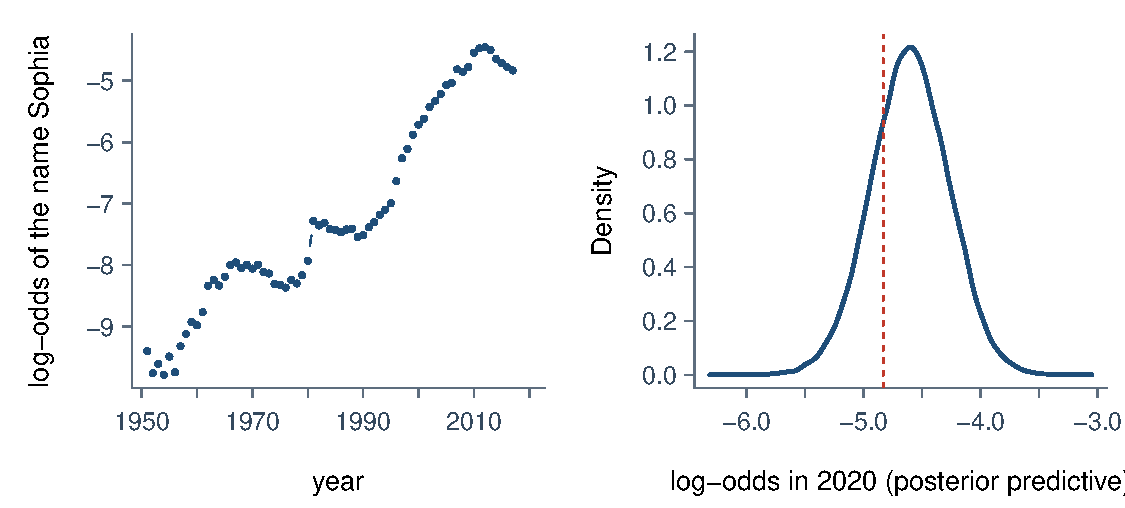
\includegraphics[width=0.98\linewidth]{ex09_series.pdf}\end{center}
PPD for 2020: log-odds mean $-4.60$, 95\% interval $(-5.25,\ -3.95)$; on the proportion scale, median 0.99\% of girls, 95\% interval (0.52\%, 1.88\%).

\begin{answer}
(a) $\alpha$ = trend level in 1950, $\beta$ = trend slope per year, $\rho$ = persistence of deviations, $\sigma^2$ = shock variance. (b) $\rho\approx0.99$ (95\% CI 0.91--1.00), $\sigma\approx0.18$; $\alpha$ and $\beta$ are poorly determined because the series is close to a random walk; JAGS agrees. (c) 2020 log-odds $\approx-4.6$ $(-5.25,-3.95)$, i.e.\ about 1\% of girls (0.5--1.9\%).
\end{answer}

\begin{takeaway}
When $\rho\approx1$, forecasts are driven by the most recent value, not by a long-run trend --- and their uncertainty grows quickly with the horizon.
\end{takeaway}

% ================================================================= Exercise 10
\exercise{4.10 --- A B-spline curve for global temperature}

\begin{problem}{10}
The global mean temperature anomaly (difference between current year and the 1951-1980 average) data on the course website and plotted in Figure 3.4. Let $X_i$ and $Y_i$ be the year and temperature anomaly (C) for observation $i$. We will analyze these data using a nonparametric regression model $Y_i=g(X_i)+\varepsilon_i$ as in Section 8.3, where $g$ is modeled as a linear combination of $J=15$ B-spline basis functions.
\begin{enumerate}[(a)]
\item Fit the model, and plot the data along with the posterior mean and 95\% posterior interval of $g(X_i)$ for each value $X_i$.
\item Summarize and interpret the posterior distribution of $\Delta=g(2020)-g(1980)$.
\item Summarize and interpret the posterior distribution for $\delta_i=g(X_i)-g(X_{i-1})$ for each $i>1$.
\end{enumerate}
\end{problem}

\begin{restate}
Fit a smooth curve to 142 yearly temperature anomalies, measure the warming between 1980 and 2020, and estimate the warming rate in each year.
\end{restate}

\begin{recall}
\textbf{B-splines}: $J$ smooth ``bump'' functions $B_1(x),\dots,B_J(x)$ spread over the range of $x$. Writing $g(x)=\sum_{j=1}^J\beta_jB_j(x)$ turns curve fitting into \emph{linear regression} on the $J$ columns $B_j(X_i)$ (R: \texttt{splines::bs(year, df = 15, intercept = TRUE)}). Any function of $g$ (differences, maxima) has a posterior obtained by applying it to each draw of $\bm\beta$.
\end{recall}

\begin{keyidea}
Gibbs sampler for linear regression on the 15 basis columns; for each draw compute the whole curve $g(X_1),\dots,g(X_{142})$, then $\Delta$ and the $\delta_i$.
\end{keyidea}

\solution
\step{(a) Fit.} Data: 1880--2021. Priors $\beta_j\sim\dist N(0,100^2)$, $\sigma^2\sim\dist{InvGamma}(0.01,0.01)$; 10{,}000 kept draws. Residual SD $\sigma\approx0.099^\circ$C.
\begin{center}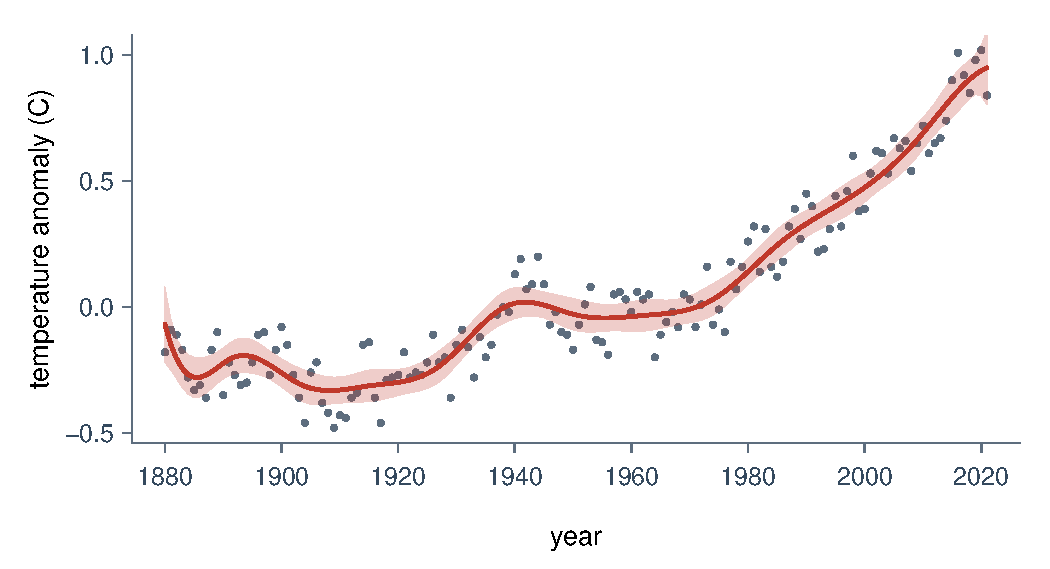
\includegraphics[width=0.85\linewidth]{ex10_curve.pdf}\end{center}
The curve shows slight cooling to $\approx1910$, warming to the 1940s, a plateau to the 1970s, then rapid warming.

\step{(b) $\Delta=g(2020)-g(1980)$.}
For each draw, subtract the curve values at 1980 and 2020: posterior mean $\mathbf{0.80^\circ C}$, 95\% interval $(0.69,\ 0.91)$, $\Prob(\Delta>0\mid\text{data})>0.9999$. The trend (not just the noisy yearly values) warmed by about $0.8^\circ$C in 40 years --- roughly $0.2^\circ$C per decade.

\step{(c) Year-to-year changes $\delta_i$.}
\begin{center}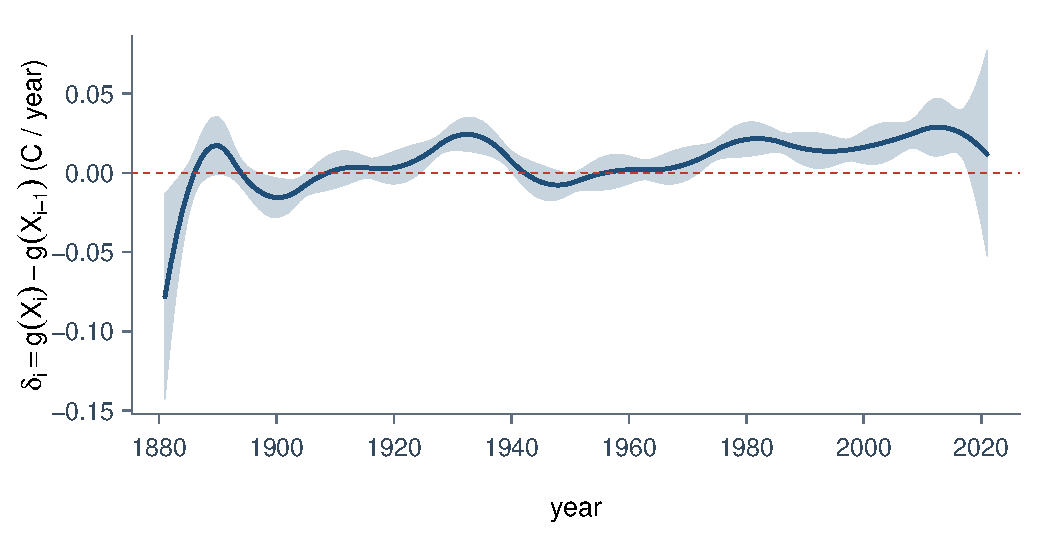
\includegraphics[width=0.85\linewidth]{ex10_rate.pdf}\end{center}
The posterior mean rate peaks at $0.029^\circ$C/year (2013). In 67 of the 141 years the posterior probability of warming ($\delta_i>0$) exceeds 0.95, including every year from 1972 to 2018. The interval for the last year (2021: $0.012$, 95\% CI $(-0.053,\ 0.077)$) is wide: splines are least certain at the ends of the data.

\begin{answer}
(a) See figure: a smooth curve with a narrow 95\% band. (b) $\Delta\approx0.80^\circ$C (95\% CI 0.69--0.91): warming between 1980 and 2020 is certain. (c) The warming rate has been positive with posterior probability above 0.95 in every year from 1972 to 2018, peaking around $0.03^\circ$C/year; rates for 2019--2021 are uncertain (edge effect).
\end{answer}

\begin{takeaway}
Bayesian inference gives uncertainty for \emph{any} derived quantity (differences, derivatives, maxima) for free --- just compute it draw by draw.
\end{takeaway}

% ================================================================= Exercise 11
\exercise{4.11 --- When to use which prior: marine biodiversity}

\begin{problem}{11}
Consider an ecological study where the response, $Y_i$, is a measure of marine biodiversity at location $i=1,\dots,n$. The covariates $X_{i1},\dots,X_{ip}$ are summaries of the environment of location $i$, such as water depth, distance to shore, fishing regulations, etc. Assume the multiple linear regression model $Y_i=\beta_0+X_{i1}\beta_1+\dots+X_{ip}\beta_p+\varepsilon_i$. Give a scenario where the following priors for the $\beta_j$ might be useful:
\begin{enumerate}[(a)]
\item Jeffreys prior
\item Bayesian LASSO prior
\item An informative prior $\beta_j\sim\dist{Normal}(m_j,v)$ for small $v$
\end{enumerate}
Your scenarios should include both numerical summaries such as $n$ and $p$ and scientific objectives.
\end{problem}

\begin{restate}
Describe a realistic study in which each kind of prior is the natural choice.
\end{restate}

\begin{recall}
\begin{itemize}
\item \textbf{Jeffreys} (flat on $\bm\beta$, $1/\sigma^2$ on the variance): objective; reproduces least squares; needs $n\gg p$.
\item \textbf{Bayesian LASSO} (double exponential): shrinks small coefficients toward 0; for many candidate predictors.
\item \textbf{Informative} $\dist N(m_j,v)$: encodes reliable outside knowledge.
\end{itemize}
\end{recall}

\begin{keyidea}
Match the prior to (i) how many covariates there are relative to the sample size and (ii) what is already known.
\end{keyidea}

\solution
\step{(a) Jeffreys prior.}
\emph{Scenario}: a large monitoring programme with $n=800$ reef sites and $p=4$ pre-specified covariates (depth, distance to shore, protection status, water temperature). \emph{Objective}: an impartial estimate of the effect of marine protected areas, to be reported to a regulator. With $n/p=200$ the data dominate and an objective prior avoids any accusation that the conclusions were ``built into'' the prior.

\step{(b) Bayesian LASSO.}
\emph{Scenario}: $n=60$ sites with $p=45$ candidate environmental summaries (depth, slope, salinity, 10 nutrient measures, 20 satellite indices, fishing pressure, \ldots), many of them correlated. \emph{Objective}: identify which few factors drive biodiversity and build a predictive map. With $p$ close to $n$ least squares is unstable; the LASSO prior shrinks the many negligible effects toward zero and stabilises the important ones.

\step{(c) Informative prior with small $v$.}
\emph{Scenario}: a small pilot study, $n=12$ sites in a new region, $p=3$ (depth, distance to shore, protection). A meta-analysis of 40 earlier studies estimated the depth effect precisely, giving $m_{\text{depth}}$ and a small $v$. \emph{Objective}: estimate the protection effect in the new region. With only 12 sites, borrowing the well-established depth effect frees the scarce data to inform the protection effect.

\begin{answer}
(a) Jeffreys: large $n$ (e.g.\ 800), few pre-specified $p$ (4), objective reporting. (b) Bayesian LASSO: $p$ near $n$ (45 vs 60), variable selection/prediction. (c) Informative: tiny new study ($n=12$, $p=3$) plus strong external evidence on some effects.
\end{answer}

\begin{takeaway}
The prior is part of the study design: it should reflect the ratio $p/n$ and the existing scientific knowledge.
\end{takeaway}

% ================================================================= Exercise 12
\exercise{4.12 --- Genetic markers for depression}

\begin{problem}{12}
In a study of the genetic determinants of depression, researchers gathered information from 1000 patients. The response variable is the (continuous) CES-D survey score and the predictors 10,000 genetic markers. The objective is to determine if any of the markers are associated with depression.
\begin{enumerate}[(a)]
\item Describe and justify a model and prior for these data
\item How would you summarize the results?
\end{enumerate}
\end{problem}

\begin{restate}
1{,}000 patients but 10{,}000 possible predictors: design a Bayesian model that can find the few markers (if any) that matter.
\end{restate}

\begin{recall}
\textbf{Spike-and-slab prior}: $\beta_j=\gamma_j\,b_j$ with $\gamma_j\sim\dist{Bernoulli}(q)$ (``is marker $j$ active?'') and $b_j\sim\dist N(0,v)$. The posterior inclusion probability $\Prob(\gamma_j=1\mid\mathbf Y)$ measures the evidence for marker $j$. Continuous alternatives: horseshoe or Bayesian LASSO priors.
\end{recall}

\begin{keyidea}
With $p=10n$, least squares is impossible; the prior must encode \emph{sparsity}: most markers have no effect.
\end{keyidea}

\solution
\step{(a) Model.}
\[
Y_i=\beta_0+\sum_{k}W_{ik}\eta_k+\sum_{j=1}^{10{,}000}G_{ij}\beta_j+\varepsilon_i,\qquad\varepsilon_i\iid\dist N(0,\sigma^2),
\]
where $Y_i$ is the CES-D score (possibly log-transformed, since it is skewed and bounded), $G_{ij}$ the standardised genotype (0/1/2 copies of the minor allele), and $W_{ik}$ \textbf{confounders} that must not be shrunk: age, sex, and the first few genetic principal components (to adjust for ancestry, which otherwise creates spurious associations).
\step{(a) Priors.}
\begin{itemize}
\item Markers: spike-and-slab $\beta_j=\gamma_jb_j$, $\gamma_j\sim\dist{Bernoulli}(q)$, $b_j\sim\dist N(0,v)$, with $q\sim\dist{Beta}(1,1000)$ so that \emph{a priori} only $\approx10$ markers are expected to be active, and the data can learn $q$ (this automatically adjusts for multiplicity).
\item Confounders and intercept: vague normal priors; $\sigma^2$: vague inverse-gamma.
\end{itemize}
\emph{Justification}: genetic effects on complex traits are typically few and small; the sparsity prior prevents over-fitting and shares information across markers about how many are active.

\step{(b) Summaries.}
\begin{itemize}
\item A Manhattan-style plot of the posterior inclusion probabilities $\Prob(\gamma_j=1\mid\mathbf Y)$ along the genome.
\item A list of markers with high inclusion probability, chosen to control the \textbf{Bayesian false discovery rate} (e.g.\ the largest set whose average $1-\Prob(\gamma_j=1\mid\mathbf Y)$ is below 5\%), with posterior means and 95\% intervals of their effects.
\item The posterior of $q$ (how many markers are active) and of the variance explained by genetics.
\item If nothing passes the threshold, say so: ``no marker shows convincing evidence of association''.
\end{itemize}

\begin{answer}
(a) Linear regression of (transformed) CES-D on standardised markers plus unshrunk confounders (age, sex, ancestry PCs), with a sparsity-inducing spike-and-slab (or horseshoe) prior and a learned inclusion rate. (b) Posterior inclusion probabilities (plot along the genome), a Bayesian-FDR-controlled list of markers with effect estimates, and the posterior number of active markers.
\end{answer}

\begin{takeaway}
In high dimensions, the prior \emph{is} the regularisation. Learning the sparsity level from the data is what makes the Bayesian approach handle multiple testing automatically (Chapter 5).
\end{takeaway}

% ================================================================= Exercise 13
\exercise{4.13 --- A three-component normal mixture for the galaxies}

\begin{problem}{13}
Open and plot the galaxies data in R using the code below,
\begin{lstlisting}
> library(MASS)
> data(galaxies)
> ?galaxies
> Y <- galaxies
> hist(Y,breaks=25)
\end{lstlisting}
Model the observations $Y_1,\dots,Y_{82}$ using a mixture of $K=3$ normal distributions. For each of the $S$ MCMC iterations evaluate the density function on the grid $y\in\{5000,5100,\dots,40000\}$ (351 points in the grid), giving an $S\times351$ matrix of posterior samples. Plot the posterior median and 95\% credible set of the density function at each of the 351 grid values. Does this mixture model fit the data well?
\end{problem}

\begin{restate}
Fit a mixture of three bell curves to the galaxy velocities and show the fitted density with its uncertainty.
\end{restate}

\begin{recall}
\textbf{Mixture model with latent labels}: $z_i\in\{1,2,3\}$ says which component galaxy $i$ belongs to; $\Prob(z_i=k)=w_k$, $Y_i\mid z_i=k\sim\dist N(\mu_k,\sigma_k^2)$. Gibbs sampler: (1) $\Prob(z_i=k\mid\cdot)\propto w_k\phi(Y_i;\mu_k,\sigma_k^2)$; (2) $\mathbf w\mid\mathbf z\sim\dist{Dirichlet}(1+n_1,1+n_2,1+n_3)$; (3) $\mu_k,\sigma_k^2$ updated from the galaxies currently in component $k$ (normal and inverse-gamma).
\end{recall}

\begin{keyidea}
The density $f(y)=\sum_kw_k\phi(y;\mu_k,\sigma_k^2)$ is a function of the parameters, so each MCMC draw gives one whole curve. Percentiles across the $S$ curves give the band. (Label switching does not matter for the density.)
\end{keyidea}

\solution
\step{Set-up.} Velocities in 1{,}000 km/s. Priors: $\mu_k\sim\dist N(20,10^2)$, $\sigma_k^2\sim\dist{InvGamma}(1,1)$, $\mathbf w\sim\dist{Dirichlet}(1,1,1)$. 20{,}000 iterations, 5{,}000 burn-in: an $S\times351$ matrix with $S=15{,}000$.
\step{Component estimates} (sorted by mean):
\begin{center}
\begin{tabular}{lccc}\toprule
Component & mean $\mu_k$ (1000 km/s) & SD $\sigma_k$ & weight $w_k$\\\midrule
1 & 9.72 (9.17, 10.28) & 0.71 & 0.09\\
2 & 21.37 (20.84, 21.90) & 2.20 & 0.85\\
3 & 32.29 (25.30, 34.48) & 1.77 & 0.06\\\bottomrule
\end{tabular}
\end{center}
\step{Fitted density.}
\begin{center}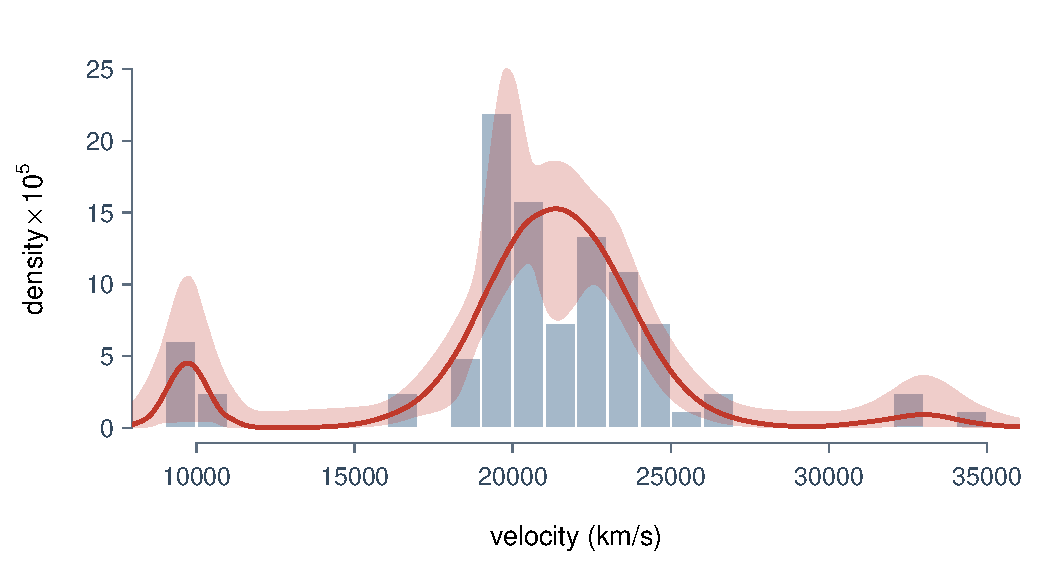
\includegraphics[width=0.85\linewidth]{ex13_mixture.pdf}\end{center}
\step{Does it fit?} \textbf{Much better} than the single $t$ (Exercise 3.9) or Laplace (Exercise 3.10): the small clusters near 10{,}000 and 33{,}000 km/s now get their own components. It is still not perfect: the large central component smooths over visible structure between 16{,}000 and 26{,}000 km/s (the histogram has two or three bumps there), so $K=4$--6 would likely fit better.

\begin{answer}
The three components sit at about 9{,}700, 21{,}400 and 32{,}300 km/s with weights 0.09, 0.85, 0.06. The posterior median density and 95\% band track the histogram well, including both outer clusters; the remaining misfit is sub-structure inside the main cluster, suggesting more components.
\end{answer}

\begin{takeaway}
Mixtures are a flexible way to model multi-modal data. Choosing $K$ is a model-selection question (Chapter 6).
\end{takeaway}

% ================================================================= Exercise 14
\exercise{4.14 --- Designing a habitat model for woodpeckers}

\begin{problem}{14}
A group of 10 ecologists is surveying a forest for Red Cockaded Woodpeckers (RCP). Each ecologist will walk along a different path and make 25 stops. At each stop, they will record local conditions (tree density, elevation, etc.) and whether they see or hear an RCP. The objective is to build a model for the types of habitat that are the most favorable to the RCP.
\begin{enumerate}[(a)]
\item Describe and justify a model and prior for these data
\item How would you summarize the results?
\end{enumerate}
\end{problem}

\begin{restate}
250 yes/no observations (10 paths $\times$ 25 stops) with habitat covariates. Design a Bayesian model that finds the best habitat while accounting for who did the survey and where.
\end{restate}

\begin{recall}
\begin{itemize}
\item Binary outcomes $\Rightarrow$ logistic regression.
\item Stops on the same path (same ecologist, nearby locations) are correlated $\Rightarrow$ random effects (Exercise 8).
\item \textbf{Imperfect detection} (Exercise 1.15): ``not seen'' does not mean ``absent''.
\end{itemize}
\end{recall}

\begin{keyidea}
Separate \emph{where the birds live} (habitat) from \emph{how good each ecologist is at spotting them} (detection).
\end{keyidea}

\solution
\step{(a) Model.} For stop $j$ on path $i$, $Y_{ij}=1$ if an RCP is seen or heard. A simple and defensible choice is a logistic mixed model
\[
\mathrm{logit}\,\Prob(Y_{ij}=1)=\beta_0+\sum_k X_{ijk}\beta_k+u_i,\qquad u_i\iid\dist N(0,\tau^2),
\]
with $X_{ijk}$ the standardised habitat covariates (tree density, elevation, tree age, understory, \ldots). The path/ecologist effect $u_i$ absorbs differences in observer skill and in the part of the forest each path covers. Because consecutive stops are close in space, one can add a spatially correlated term (e.g.\ an AR(1) effect along the path) if residuals are correlated.

\emph{Better (occupancy) version}: write $Y_{ij}=Z_{ij}D_{ij}$ with occupancy $Z_{ij}\sim\dist{Bernoulli}(\psi_{ij})$, $\mathrm{logit}\,\psi_{ij}=\mathbf X_{ij}\bm\beta$ (habitat), and detection $D_{ij}\sim\dist{Bernoulli}(p_i)$ with an ecologist-specific detection probability $p_i$. Repeat visits to some stops make $\psi$ and $p$ separately identifiable.
\step{(a) Priors.} $\beta_k\sim\dist N(0,2.5^2)$ on standardised covariates (weakly informative: odds ratios beyond $e^{5}$ per SD are implausible, which also prevents separation problems with 250 binary outcomes); $\tau\sim$ half-normal(0,1) or $\tau^2\sim\dist{InvGamma}(0.1,0.1)$; detection $p_i\sim\dist{Beta}(2,2)$. If a previous RCP study exists, its estimates can inform the habitat priors.

\step{(b) Summaries.}
\begin{itemize}
\item Posterior means and 95\% intervals of the odds ratios $e^{\beta_k}$ for each habitat variable, and $\Prob(\beta_k>0\mid\mathbf Y)$.
\item The posterior of $\tau$ (how much paths/observers differ) and of each ecologist's detection probability.
\item Predicted occupancy probability $\psi$ as a function of the key habitat variables (partial-effect curves), and a map of predicted suitability over the forest, with uncertainty.
\item Posterior predictive checks (e.g.\ number of detections per path) to confirm the model fits.
\end{itemize}

\begin{answer}
(a) A logistic regression of detection on standardised habitat covariates with a random effect for path/ecologist (ideally an occupancy model separating habitat-driven occupancy from observer-specific detection), with weakly informative $\dist N(0,2.5^2)$ priors. (b) Odds ratios with intervals, observer/path variation, predicted occupancy curves and a habitat-suitability map with uncertainty, plus posterior predictive checks.
\end{answer}

\begin{takeaway}
Survey data carry the fingerprints of the people who collected them; a good model separates the biology from the observation process.
\end{takeaway}

\end{document}
